% concatenated from ITT.tex, Picture_1.tex

\documentclass[12pt, english]{article}
\usepackage[utf8]{inputenc}
\usepackage{amsthm}
\usepackage{amssymb}
\usepackage[all]{xy}
\usepackage{amsmath}
\usepackage{tikz-cd}
\usepackage{tikz}
\usepackage{float}
\usepackage{bbm}

\tikzcdset{scale cd/.style={every label/.append style={scale=#1},
		cells={nodes={scale=#1}}}}
\setlength{\parindent}{0pt}

\newcommand{\RNum}[1]{\uppercase\expandafter{\romannumeral #1\relax}}

\newcommand{\doublearrow}[1]{\xrightarrow[]{#1}\mathrel{\mkern-14mu}\rightarrow}


\usepackage{rotating}
\usepackage{caption, booktabs}
\usepackage{verbatim}
%\usepackage[active,tightpage]{preview}
%\PreviewEnvironment{tikzpicture}
%\setlength{\PreviewBorder}{10pt}%
\usetikzlibrary{calc}


\usepackage{tikz}
\usetikzlibrary{patterns}

\usepackage{pdflscape}

\usepackage{mathtools}
\usepackage[english]{babel}
%\usepackage{MnSymbol}
\usepackage{enumitem}
%\usepackage{breqn}


\usepackage{hyperref}
\usepackage{bookmark}




\newtheorem{definition}{Definition}[section]
\newtheorem{beispiel}[definition]{Beispiel}
\newtheorem{proposition}[definition]{Proposition}
\newtheorem{remark}[definition]{Remark}
\newtheorem{lemma}[definition]{Lemma}
\newtheorem{satz}[definition]{Satzas hypersurfaces in toric varieties}
\newtheorem{theorem}[definition]{Theorem}
\newtheorem{corollar}[definition]{Corollary}
\newtheorem{construction}[definition]{Construction}
\newtheorem{facts}[definition]{Facts}
\newtheorem{example}[definition]{Example}
\newtheorem{consequence}[definition]{Consequence}
\newtheorem{condition}[definition]{Condition}
\newtheorem{conjecture}[definition]{Conjecture}

\DeclareMathOperator{\ord}{ord}
\DeclareMathOperator{\Hom}{Hom}
\DeclareMathOperator{\Pic}{Pic}
\DeclareMathOperator{\coker}{coker}
\DeclareMathOperator{\Lie}{Lie}
\DeclareMathOperator{\Aut}{Aut}
\DeclareMathOperator{\Gl}{Gl}
\DeclareMathOperator{\Codim}{Codim}
\DeclareMathOperator{\res}{res}
\DeclareMathOperator{\Cl}{Cl}
\DeclareMathOperator{\rk}{rk}
\DeclareMathOperator{\Gr}{Gr}
\DeclareMathOperator{\ind}{ind}
\DeclareMathOperator{\Ext}{Ext}
\DeclareMathOperator{\lcm}{lcm}
\DeclareMathOperator{\Vol}{Vol}
\DeclareMathOperator{\Stab}{Stab}
\DeclareMathOperator{\Int}{Int}
\DeclareMathOperator{\Min}{Min}
\DeclareMathOperator{\Supp}{Supp}
\DeclareMathOperator{\Bound}{Bound}
\DeclareMathOperator{\Cone}{Cone}
\DeclareMathOperator{\Convhull}{Convhull}


\begin{document}

	\title{Jacobian rings and the infinitesimal Torelli Theorem}
\author{Julius Giesler,\\ University of T\"ubingen}
\date{\today}
\maketitle
\begin{abstract}
	In this article we deal with jacobian rings and identify a mixed Hodge component of a nondegenerate hypersurface in the torus with a lattice geometric quotient vector space. We introduce a period map, study its differential and compute the kernel of the differential much explicitly via certain Laurent polynomials. As a main application we deal with the infinitesimal Torelli theorem (ITT). We study the kernel of the cohomological map for explicit deformations and complete our study by dealing with the remaining part $\coker(\kappa_{\mathbb{P},f})$ (cokernel of the Kodaira-Spencer map) in dimensions $n \geq 4$.
\end{abstract}

\section{Introduction}

Being a subsequent paper to the paper (\cite{Gie22}) summarizing, generalizing and extending results from my doctoral thesis (\cite{Gie23}) we adopt the notation respectively. Given a \textit{nondegenerate} Laurent polynomial 
\begin{align} \label{represenation_f_intro}
	f = \sum\limits_{m \in \Delta \cap M} a_m \cdot x^m
\end{align}
with $n$-dimensional Newton polytope $\Delta$ take 
\[ Z_f := \{ f=0 \} \subset T. \]

\begin{comment}
We are looking for a good compactification of $Z_f$ realized as closure in a suitable projective toric variety. The Newton polytope $\Delta$ of $f$ defines a projective toric variety $\mathbb{P}_{\Delta}$ via its normal fan and there is a diagram
\begin{equation*}
	\begin{tikzcd}
		& \overbrace{\tilde{Z}_f}^{= \textrm{ smooth compactification of } Z_f} \arrow[d, "p"] \arrow[r, phantom, sloped, "\subseteq"] & \tilde{\mathbb{P}} \arrow[d, "p"] \\
		Z_f \arrow[r, phantom, sloped, "\subseteq"] & \underbrace{Z_{\Delta,f}}_{= \textrm{ closure of } Z_f \textrm{ in } \mathbb{P}_{\Delta}} \arrow[r, phantom, sloped, "\subseteq"] & \mathbb{P}_{\Delta}
	\end{tikzcd}
\end{equation*}

where $p$ denotes a toric resolution of singularities and $\tilde{Z}_f$ the preimage of $Z_{\Delta,f}$ under $p$. In $1986$ Vladimir I. Danilov and Askold G. Khovanskii invented ideas how the \textit{Hodge-Deligne numbers} of $Z_f$ and the \textit{Hodge numbers} of $\tilde{Z}_f$ could be calculated. In examples this program works nice in lower dimensions or if the normal fan $\Sigma_{\Delta}$ of $\Delta$ is simplicial. 
\leavevmode
\\
Criticism:
\end{comment}

%\begin{itemize}
%	\item 


%	\item The authors stay somehow \glqq loose\grqq \, in specifying a nice compactification of $Z_f$: They do not construct or deal with special compactifications, that are of great importance in higher-dimensional algebraic geometry, though their methods are quite general and if $\Sigma_{\Delta}$ is simplicial the compactification $Z_{\Delta,f}$ is already useful enough for the calculations of the Hodge numbers. This is improved in (\cite{Bat22}) by constructing a minimal compactification $Y_f \subset \mathbb{P}$. %: There it is constructed a projective toric variety $\mathbb{P}$ to a fan $\Sigma$, such that the closure $Z_f \subset Y_f \subset \mathbb{P}$ of $Z_f$ gets a {\bf minimal model} of $Z_f$, that is $Y_f$ has terminal singularities and $K_{Y_f}$ is nef.
%\end{itemize}


We are interested in the mixed Hodge components 
	\begin{align} \label{equation_mixed_Hodge_components_of_Z_f_of_min_wei}
		H^{n-k,k-1} H^{n-1}(Z_f, \mathbb{C}) \cong R_{Int,f}^{k}
	\end{align}
	of weight $n-1$ and their dimensions, where $R_{Int,f}^k$ denotes a graded component of an \textit{interior module} defined via jacobian rings (of Batyrev), (see \cite{Bat93}). The isomorphism (\ref{equation_mixed_Hodge_components_of_Z_f_of_min_wei}) identifies the mixed Hodge components of minimal weight with vector spaces defined by the lattice geometry of integral multiples of $\Delta$ (definition \ref{definition_R_Int_f_k}). In this article we find a representation of $R_{Int,f}^k$ as quotient vector space that illustrates Griffiths concept of \textit{(infinitesimal) variation of Hodge structure} for toric hypersurfaces: (Proposition \ref{proposition_Hodge_comp_Z_f_arbitary_k_dimensions_and_basis})

\begin{proposition} \label{proposition_Hodge_comp_Z_f_arbitary_k_dimensions_and_basis_intro}
	Let $\Delta$ be an $n$-dimensional lattice polytope with $l^*(\Delta) > 0$ and a given $f$. Given $\Gamma_1,...,\Gamma_{n+1} \leq \Delta$ with $n_{\Gamma_1},...,n_{\Gamma_{n+1}}$ affine linear independent. Then 
	\begin{align*}
		L^*(k \cdot \Delta) / U_{f,k} = R_{Int,f}^k \quad k=1,...,n
	\end{align*}
	where $U_{f,k}$ denotes the vector space over $\mathbb{C}$ spanned by
	\begin{align}
		& g_{\Gamma_i}(f) \cdot x^v \quad i=1,...,n+1, \quad v \in \Int((k-1) \cdot \Delta) \cap M \label{formula_relation_g_Gamma_i_f_the_1}	 \\
		& g_{\Gamma}(f) \cdot x^v \quad \Gamma \leq \Delta, \quad \quad \quad \quad \, \, \, \, v \in \Int((k-1) \cdot \Gamma) \cap M \label{formula_relation_g_Gamma_i_f_the_2}
	\end{align}
	with certain Laurent polynomials $g_{\Gamma}(f)$. For $k=2$ these relations are linear independent. Here $\Int$ denotes the relative interior and $L^*(k \cdot \Delta)$ the $\mathbb{C}$-vector space with basis $x^m$, where $m \in \Int(k \cdot \Delta) \cap M$.
\end{proposition}

The $g_{\Gamma}(f)$'s in fact are useful generators of the first component $J_{\Delta,f}^1$ of the jacobian ideal. %These formulas rely on the nondegeneracy of $f$ which could be translated in an algebraic independence between certain Laurent polynomials $F_0,...,F_n$ (see theorem \ref{theorem_characterization_Delta_regular}). 
Using a resolution of the vector space $R_{Int,f}^k$ we were able to specify a complete list of relations between the above generators for $k > 2$.
%A deficit is that the above generators of $U_{f,k}$ are almost never linearly independent for $k \geq 3$.
\leavevmode
\\


%\underline{\bf The period map and the ITT (infinitesimal Torelli theorem)} \leavevmode \\ \\

We then introduce the usual period map $\mathcal{P}_{B,f}$ with entries
%Varying $f$ we are keen to know whether the Hodge components of $H^{n-1}(Y_f,\mathbb{C})$ determine $Y_f$ in the family $\mathcal{X} \rightarrow B$ up to isomorphism. One could make this problem precise by introducing and studying properties of the \textit{period map} $\mathcal{P}_{B,f}$.  This leads to so called \textit{Torelli type Theorems}. These are not really \glqq uniform Theorems\grqq \, as there are algebraic varieties failing them, but such varieties are often very exceptional. We restrict to the \textit{infinitesimal Torelli Theorem} for $\mathcal{X} \rightarrow B$. The period map $\mathcal{P}_{B,f}$ with entries
\begin{align*}
	\mathcal{P}_{B,f}^k: f' \mapsto F^{k}H^{n-1}(Y_{f'},\mathbb{C}) \subset H^{n-1}(Y_f,\mathbb{C})
\end{align*}
with $\{ F^k \}$ the Hodge filtration. This map is known to be holomorphic. The $k$-th component $d \mathcal{P}_{B,f}^k$ of the differential $d \mathcal{P}_{B,f}$ factors as follows
\begin{equation}
	\begin{tikzcd} \label{Commutative_diagram_Kodaira_Spencer_map_dP_intro}
		T_{B,f}  \arrow[swap]{dr}{d \mathcal{P}_{B,f}^k } \arrow{r}{\kappa_{f}} & H^{1}(Y_f,T_{Y_f})  \arrow{d}{\Phi_f^k} \\
		& \Hom(H^{k}(Y_f, \Omega_{Y_f}^{n-1-k}), H^{k+1}(Y_f, \Omega_{Y_f}^{n-2-k}))
	\end{tikzcd}
\end{equation}
Our idea is strainghtforward: Compute the kernel $\ker(d \mathcal{P}_{B,f})$ and compare it with $\ker(\kappa_f)$, which we explicitly computed in the preceeding article \cite{Gie22}, to finally deduce on $\ker(\Phi_{f \vert{Im(\kappa_f)}})$. A detailed study of the components $R_{Int,f}^k$ and the relations between the generators of $0 \in R_{Int,f}^k$ gives the following key result (theorem \ref{Theorem_formula_ker_ITT})
%conjecture on the kernel of $d \mathcal{P}_{B,f}$ which though we do not prove:


\begin{theorem} \label{Theorem_formula_ker_ITT_intro}
	Let $\Delta$ be an $n$-dimensional lattice polytope with $(0,...,0) \in \Int(\Delta) \cap M$. If $f \in L(\Delta)$ is generic (varying in a nonempty Zariski open subset) then
	\begin{align} \label{general_formula_for_ker_DP_MDelta_handable_intro}
		\ker(d \mathcal{P}_{B,f}^1) \overset{\mod \Lie(T)}{=}&  \Big\langle g_{\Gamma}(f) \cdot x^w \in L(\Delta)/\mathbb{C} \cdot f \quad \mid \quad  \Gamma \leq \Delta \textrm{ a facet}, \nonumber  \\
		& w + v \in \big( \Int(\Delta) \cup \Int(\Gamma) \big) \cap M, \nonumber \quad \\ 
		& \forall \, v \in \Int(\Delta) \cap M \Big\rangle. \nonumber
	\end{align}
	where $\langle \rangle$ denotes the span as $\mathbb{C}$-vector space.
\end{theorem}

This direct approach to the diagram of Griffiths (\ref{Commutative_diagram_Kodaira_Spencer_map_dP_intro}) is not published yet and yields a both computational and much explicit perspective. 
%Given the assumptions of the theorem we easily deduce
%If conjecture (\ref{Theorem_formula_ker_ITT_intro}) is true for $k=1,...,n-1$ 
%\begin{align*}
%	\ker(d \mathcal{P}_{B,f}^k) = \ker(d \mathcal{P}_{B,f}^1), \quad k \geq 1
%\end{align*}
%(Corollary \ref{corollary_conjecture_ker_dphi_f_k}). 
\leavevmode 
\\
Let $g = g_{\Gamma}(f) \cdot x^w \in \ker(d \mathcal{P}_{B,f}^1)$. Then we get the distinction
\begin{equation} \label{distinction_scalar_product_0_minus1_getminus2}
	\begin{tikzcd}
		\langle w,n_{\Gamma} \rangle = \left\{\begin{array}{lll} 0, & \Leftrightarrow g \equiv 0 \\
			-1, &  \Leftrightarrow g \in \ker(\kappa_f) \\
			\leq -2, & \quad \, \, \textrm{exceptional cases}
		\end{array}\right.
	\end{tikzcd}
\end{equation}
and $\langle w,n_{\Gamma'} \rangle \geq 0$ for $\Gamma' \neq \Gamma$ by Theorem (\ref{Theorem_formula_ker_ITT_intro}) with $n_{\Gamma}$ the inner facet normal to $\Gamma$. The last case in the distinction causes $\Phi_{f \vert{Im \, \kappa_f}}$ to be not injective, which implies that the infinitesimal Torelli theorem (ITT) fails for such hypersurfaces $Y_f$. %\leavevmode \\ \\
%For smooth projective hypersurfaces $Y_f \subset \mathbb{P}^n$ of degree $\geq n+2$, where $n \geq 3$ the Kodaira-Spencer map $\kappa_f$ is surjective and we use this to get a new proof of the ITT for such nondegenerate hypersurfaces. We then finish with the following corollary
\begin{corollar}
	Given $\Int(\Delta) \cap M \nsubseteq \{\textrm{plane}\}$ and $f \in L(\Delta)$ generic (and nondegenerate) then $\ker(d \mathcal{P}_{B,f}) = \ker(\kappa_f)$. Thus
\[  \ker(\Phi_{f \vert{Im \, \kappa_f}}) = \{ 0  \},  \]
We say that $Y_f$ fulfills the ITT for $\mathcal{X} \rightarrow B$.  
\end{corollar}

This corollary follows easily from above: Namely we construct a $3$-dimensional empty polytope $Q$ with $6$ vertices. $Q$ is the convex span of an empty triangle with vertex $(0,0,0)$ and this triangle dilated by $w$. Then we use a theorem of White on empty $3$-simplices to deduce $|Q \cap M| \geq 7$ under the assumption $\langle w,n_{\Gamma} \rangle \leq -2$, a contradiction.
\leavevmode 
\\ 
%Concerning the cokernel $\coker(\kappa_{f})$ the situation might get more complicated, see also \cite[Cor.7.1]{Gie22}. In (\cite{Mav03}) there were made some efforts for $Y_f$ a K3 hypersurface (so called non-polynomial deformations), realizing these deformations as deformations of complete intersections in a single big toric variety, but is seems unlikely that this representation is useful in order to compute the missing vector space $\ker(\Phi_{f \vert{\coker(\kappa_f)}})$. Besides in (\cite{BrGr12}) there were made some efforts to combine the Hodge components and their computation to the generic Picard number of the hypersurface.

Finally we tackle the homomorphism $\Phi_{f \vert{\coker \, \kappa_f}}$ in dimension $n \geq 4$: Given a \textit{functorial toric resolution} of singularities $\tilde{\mathbb{P}} \rightarrow \mathbb{P}$ we have
\begin{align*}
	H^0(\tilde{\mathbb{P}}, T_{\tilde{\mathbb{P}}}) \cong H^0(\mathbb{P}, T_{\mathbb{P}}).
\end{align*}
%smooth refinement $\tilde{\Sigma}$ of $\Sigma$ 
We write $\tilde{Y}_f$, or by abuse of notation also $Y$, for the smooth closure of $Z_f$ in $\tilde{\mathbb{P}}$. The results on the respective \textit{Kodaira Spencer map} $\kappa_{\tilde{\mathbb{P}},f}$ remain valid (section \ref{section_Kod_Sp_map_smooth_bir_model}): Up to slightly adapting $\Delta$ we get $\kappa_{\tilde{\mathbb{P}},f} = \kappa_f$ and given $n \geq 4$ we have an exact sequence
\begin{align*}
	0 \rightarrow Im(\kappa_{f}) \rightarrow H^1(\tilde{Y}, T_{\tilde{Y}}) \rightarrow H^1(\tilde{\mathbb{P}}, T_{\tilde{\mathbb{P}}}) \rightarrow 0.
\end{align*}
The cohomological map $\Phi_f$ in the infinitesimal Torelli theorem (ITT) is made up of cup product and contraction. Given $n \geq 4$ we show how $\Phi_f$ could be realized on $\coker(\kappa_{f})$ again by cup product and contraction (section \ref{section_ITT_on_coker_computation}). We then deduce on the ITT on the remaining part $\coker(\kappa_{f})$ (section \ref{section_ITT_on_coker_computation_2}) and arrive at:

\begin{theorem}
	Let $\Delta \subset M_{\mathbb{R}}$ be an $n$-dimensional lattice polytope with
	\begin{align*}
		n \geq 4, \quad \quad \Int(\Delta) \cap M \nsubseteq \textrm{ plane}
	\end{align*}
	and $f \in U_{reg}(\Delta)$ generic (with Newton polytope $\Delta$). Then the smooth birational model $Y = \tilde{Y}_f$ of $Z_f$ from above fulfills the infinitesimal Torelli theorem (ITT), that is
	\begin{align*}
		\Phi_f = \bigoplus_p \Phi_f^p: H^1(Y,T_Y) \rightarrow \bigoplus_{p} \Hom \Big( H^{n-1-p}(Y, \Omega_Y^p), H^{n-p}(Y, \Omega_Y^{p-1}) \Big)
	\end{align*}
	is injective. 
\end{theorem}

Our article relies on results from (\cite{DK86}) and (\cite{Bat93}). Let us list common methods with the authors V.I. Danilov, A.G. Khovanskii and V.V. Batyrev:
\begin{itemize}
	\item We reduce the calculation of the Hodge component $H^{n-k,k-1}(Y_f, \mathbb{C})$ to the calculation of (\ref{equation_mixed_Hodge_components_of_Z_f_of_min_wei}) (similarly to \cite{DK86}), see section \ref{Section_cohomology_affine_hypersurface_nonsingular_compactification}.
	\item We follow \cite{Bat93} to define the \textit{jacobian ring} $R_f$ and the \textit{(interior) module} $R_{Int,f}$ over $R_f$ (see section \ref{section_constr_jac_ring}) and of course use the identification (\ref{equation_mixed_Hodge_components_of_Z_f_of_min_wei}).
\end{itemize}

In section (\ref{section_smooth_and_stable_points}) we study $\Delta$ up to replacing by an integral lattice vector. In particular we effort $(0,...,0) \in \Int(\Delta)$  to build a smooth quotient of $B$ by the torus $T$.

\section{The Jacobian ring of Batyrev} \label{section_constr_jac_ring}

In the sections \ref{section_constr_jac_ring} and \ref{section_examples_comp_jac_ring_interor_module} we do not restrict to the dimension $n=3$.

\begin{definition}
	Let $\Delta$ be an $n$-dimensional lattice polytope and $S_{\Delta}$ denote the subalgebra of $\mathbb{C}[x_{0},x_{1}^{\pm},...,x_{n}^{\pm}]$  spanned as $\mathbb{C}$-vector space by $1$ and all monomials 
	\[  x_{0}^{k}x_1^{m_1}...x_{n}^{m_{n}}, \quad \textrm{where } k \in \mathbb{N}_{\geq 1},  \quad m_1,...,m_n \in \mathbb{Z}, \]
	such that the rational point
	\[ \frac{m}{k} := \Big( \frac{m_{1}}{k},...,\frac{m_{n}}{k} \Big) \]
	belongs to $\Delta$. Denote the $k$-th graded piece of $S_{\Delta}$ by $S_{\Delta}^k$.	The subalgebra $S_{\Delta}^*$ is defined in the same way except that we require that $m/k$ belongs to the interior of $\Delta$.
\end{definition}





We identify lattice points $m \in M$ with monomials $x^m \in \mathbb{C}[x_1^{\pm 1},...,x_n^{\pm 1}]$.


\begin{construction} \label{construction_Laurent_polynomials_F_i} \cite{Bat93} \\
	\normalfont
	Given a Laurent polynomial $f$ in the variables $x_1,...,x_n$ with $n$-dimensional Newton polytope $\Delta$ let
	\[ F(x_{0},x_{1},...,x_{n}) := x_{0}f(x_1,...,x_n) - 1  \]
	which is an equation for the complement $T \setminus Z_{f} \subset \overline{T}:= (\mathbb{C}^{*})^{n+1}$ of $Z_f=\{f=0\} \subset T$. Consider the logarithmic derivatives 
	\[ F_{i}(x_{0},x) := x_{i}\frac{\partial}{\partial x_{i}} F(x_{0},x) = x_i \frac{\partial (x_0 f)}{\partial x_i} \quad 0 \leq i \leq n. \]
\end{construction}
\begin{definition} \cite{Bat93} \\
	\normalfont
	The graded ideal $J_{\Delta,f}$ within $S_{\Delta}$ generated by $F_{0},...,F_{n}$ is called the \textit{jacobian ideal} and the quotient ring
	\[ R_{f} := S_{\Delta}/J_{\Delta,f} \]
	is called the \textit{Jacobian ring of Batyrev} (associated to the Laurent polynomial $f$). We denote the $k$-th homogeneous component of $R_{f}$ by $R_{f}^k$.
\end{definition}

\begin{theorem} \label{theorem_characterization_Delta_regular} \cite[Thm.4.8]{Bat93} \\
	The jacobian ring $R_{f}$ is a graded ring. It is finite dimensional as $\mathbb{C}$-vector space if and only if $f$ is nondegenerate. In this case the dimensions of $R_f^k$ are independent of the polynomial $f$. $f$ is nondegenerate if and only if $F_0,...,F_n$ are algebraically independent over $\mathbb{C}$.% and if and only if $F_0,...,F_n$ build a regular sequence in $S_{\Delta}$.
\end{theorem}



\begin{definition} \label{definition_R_Int_f_k} (\cite[Prop.9.0.6]{Bat93}) \\
	We denote the homogeneous ideal $R_f \cap S_{\Delta}^*$ of $R_{f}$ by $R_{Int,f}$ and its k-th homogeneous component by $R_{Int,f}^k$. We call $R_{Int,f}$ the \textit{interior $R_{f}$-module}. Let $D_f^k := L^*(k \cdot \Delta)/(F_0,...,F_n) \cdot L^*((k-1) \cdot \Delta)$.
\end{definition}

\begin{remark} \label{remark_duality_Poincare_duality}
	\normalfont
	Poincaré duality on $H^{n-1}(Y,\mathbb{C})$ restricts to an isomorphism
	\[ (R_{Int,f}^k)^* \cong R_{Int,f}^{n+1-k}, \quad \textrm{and } (R_{\Delta,f}^k)^* \cong D_f^{n+1-k}  \]
	by (\cite[Remark 9.5, Prop.9.7]{Bat93}). %In (\cite[Ch.9]{Bat93}) $R_{Int,f}$ is denoted by $H_f$ and should not be confused with the dualizing $R_f$-module $D_f$.
\end{remark}




%	We could dispense with the notation of $F$, writing everything only depending on $f$, but we also want to stress with this notation the fact that, similar to the jacobian ring for projective hypersurfaces, the complement, here $T \setminus Z_f$, plays a role in the identification of $R_f$ with some Hodge components. \\



\section{Construction of the components $R_{Int,f}^k$} \label{section_examples_comp_jac_ring_interor_module}



\begin{remark}
	\normalfont	
	By definition
	\[ R_{Int,f}^1 \cong L^*(\Delta) \] 
	(independently of $f$). More interestingly
	\begin{align} \label{formula_RDelta_Int_2_relations_Jf_Delta}
		R_{Int,f}^k \cong L^{*}(k \Delta) \big/ \, \Big( J_{\Delta,f}^k \cap L^{*}(k \Delta) \Big).
	\end{align}
	Since $J_{\Delta,f}^k$ is a graded ideal of $S_{\Delta}$ inductively
	\[ J_{\Delta,f}^k = L((k-1)\Delta) \cdot J_{\Delta,f}^1  \]
	\underline{Aim:} Switching to different generators of $J_{\Delta,f}^1$ allows us to describe the relations in $R_{Int,f}^k$ more explicitly.
	
\end{remark}

\begin{figure}[H]
	
	\begin{center}
		
		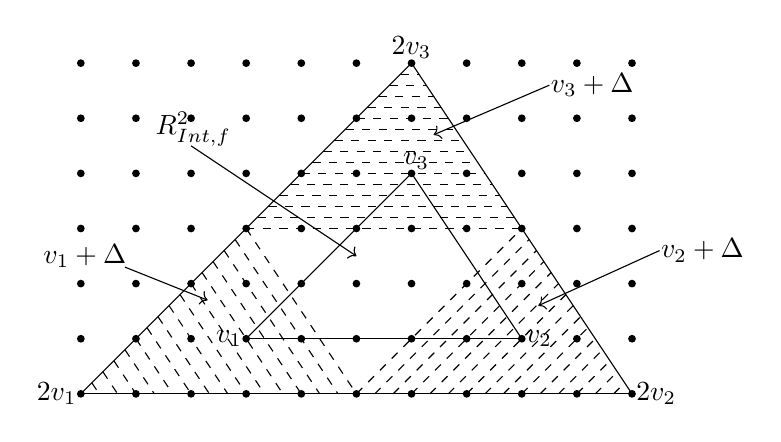
\begin{tikzpicture}[scale=0.7]
			
			
			
			\begin{scope}[xshift = 10cm]
				
				\fill (-4,0) circle(2pt);
				\fill (-4,1) circle(2pt);
				\fill (-4,2) circle(2pt);
				\fill (-4,3) circle(2pt);
				\fill (-4,4) circle(2pt);
				\fill (-4,5) circle(2pt);
				\fill (-4,6) circle(2pt);
				
				\fill (-3,0) circle(2pt);
				\fill (-3,1) circle(2pt);
				\fill (-3,2) circle(2pt);
				\fill (-3,3) circle(2pt);
				\fill (-3,4) circle(2pt);
				\fill (-3,5) circle(2pt);
				\fill (-3,6) circle(2pt);
				
				\fill (-2,0) circle(2pt);
				\fill (-2,1) circle(2pt);
				\fill (-2,2) circle(2pt);
				\fill (-2,3) circle(2pt);
				\fill (-2,4) circle(2pt);
				\fill (-2,5) circle(2pt);
				\fill (-2,6) circle(2pt);
				
				\fill (-1,0) circle(2pt);	
				\fill (-1,1) circle(2pt);
				\fill (-1,2) circle(2pt);
				\fill (-1,3) circle(2pt);
				\fill (-1,4) circle(2pt);
				\fill (-1,5) circle(2pt);
				\fill (-1,6) circle(2pt);
				
				\fill (0,0) circle(2pt);
				\fill (0,1) circle(2pt);
				\fill (0,2) circle(2pt);
				\fill (0,3) circle(2pt);
				\fill (0,4) circle(2pt);
				\fill (0,5) circle(2pt);
				\fill (0,6) circle(2pt);
				
				\fill (1,0) circle(2pt);
				\fill (1,1) circle(2pt);
				\fill (1,2) circle(2pt);
				\fill (1,3) circle(2pt);
				\fill (1,4) circle(2pt);
				\fill (1,5) circle(2pt);
				\fill (1,6) circle(2pt);
				
				\fill (2,0) circle(2pt);
				\fill (2,1) circle(2pt);
				\fill (2,2) circle(2pt);
				\fill (2,3) circle(2pt);
				\fill (2,4) circle(2pt);
				\fill (2,5) circle(2pt);
				\fill (2,6) circle(2pt);
				
				\fill (3,0) circle(2pt);
				\fill (3,1) circle(2pt);
				\fill (3,2) circle(2pt);
				\fill (3,3) circle(2pt);
				\fill (3,4) circle(2pt);
				\fill (3,5) circle(2pt);
				\fill (3,6) circle(2pt);
				
				\fill (4,0) circle(2pt);
				\fill (4,1) circle(2pt);
				\fill (4,2) circle(2pt);
				\fill (4,3) circle(2pt);
				\fill (4,4) circle(2pt);
				\fill (4,5) circle(2pt);
				\fill (4,6) circle(2pt);
				
				\fill (5,0) circle(2pt);
				\fill (5,1) circle(2pt);
				\fill (5,2) circle(2pt);
				\fill (5,3) circle(2pt);
				\fill (5,4) circle(2pt);
				\fill (5,5) circle(2pt);
				\fill (5,6) circle(2pt);
				
				\fill (6,0) circle(2pt);
				\fill (6,1) circle(2pt);
				\fill (6,2) circle(2pt);
				\fill (6,3) circle(2pt);
				\fill (6,4) circle(2pt);
				\fill (6,5) circle(2pt);
				\fill (6,6) circle(2pt);
				
				\draw (-4,0) -- (2,6);
				\draw (2,6) -- (6,0);
				\draw (6,0) -- (-4,0);
				
				\node[left] at (-1.1,4.8) {{\bf $R_{Int,f}^2$}};
				\node[left] at (-3.0,2.5) {{\bf $v_1 + \Delta$}};
				\node[right] at (6.35,2.6) {{\bf $v_2+\Delta$}};
				\node[right] at (4.35,5.6) {{\bf $v_3+\Delta$}};
				
				\node[left] at (-0.9,1) {{\bf $v_1$}};
				\node[right] at (3.9,1) {{\bf $v_2$}};
				\node[above] at (2,3.9) {{ \bf $v_3$}};
				\node[left] at (-3.9,0) {{\bf $2v_1$}};
				\node[right] at (5.9,0) {{\bf $2v_2$}};
				\node[above] at (2,5.9) {{\bf $2v_3$}};
				
				\draw[->] (-2,4.5)--(1,2.5);
				\draw[->] (-3.2,2.3) -- (-1.7,1.7);
				\draw[->] (6.5,2.6) -- (4.3,1.6);
				\draw[->] (4.5, 5.6) -- (2.4,4.7);
				
				\draw (-1,1) -- (2,4);
				\draw (2,4) -- (4,1);
				\draw (4,1) -- (-1,1);
				
				\draw[dashed] (-1,3) -- (1,0);
				\draw[dashed] (-1.2,2.8) -- (2/3,0);
				\draw[dashed] (-1.4,2.6) -- (1/3,0);
				\draw[dashed] (-1.6,2.4) -- (0/3,0);
				\draw[dashed] (-1.8,2.2) -- (-1/3,0);
				\draw[dashed] (-2.0,2.0) -- (-2/3,0);
				\draw[dashed] (-2.2,1.8) -- (-3/3,0);
				\draw[dashed] (-2.4,1.6) -- (-4/3,0);
				\draw[dashed] (-2.6,1.4) -- (-5/3,0);
				\draw[dashed] (-2.8,1.2) -- (-6/3,0);
				\draw[dashed] (-3.0,1.0) -- (-7/3,0);
				\draw[dashed] (-3.2,0.8) -- (-8/3,0);
				\draw[dashed] (-3.4,0.6) -- (-9/3,0);
				\draw[dashed] (-3.6,0.4) -- (-10/3,0);
				\draw[dashed] (-3.8,0.2) -- (-11/3,0);
				
				\draw[dashed] (-1,3) -- (4,3);
				\draw[dashed] (-0.8,3.2) -- (4-2/15,3.2);
				\draw[dashed] (-0.6,3.4) -- (4-4/15,3.4);
				\draw[dashed] (-0.4,3.6) -- (4-6/15,3.6);
				\draw[dashed] (-0.2,3.8) -- (4-8/15,3.8);
				\draw[dashed] (-0.0,4.0) -- (4-10/15,4.0);
				\draw[dashed] (0.2,4.2) -- (4-12/15,4.2);
				\draw[dashed] (0.4,4.4) -- (4-14/15,4.4);
				\draw[dashed] (0.6,4.6) -- (4-16/15,4.6);
				\draw[dashed] (0.8,4.8) -- (4-18/15,4.8);
				\draw[dashed] (1.0,5.0) -- (4-20/15,5.0);	
				\draw[dashed] (1.2,5.2) -- (4-22/15,5.2);
				\draw[dashed] (1.4,5.4) -- (4-24/15,5.4);
				\draw[dashed] (1.6,5.6) -- (4-26/15,5.6);
				\draw[dashed] (1.8,5.8) -- (4-28/15,5.8);
				
				\draw[dashed] (1.0,0) -- (4,3);
				\draw[dashed] (1+5/15,0) -- (4+2/15,2.8);
				\draw[dashed] (1+2*5/15,0) -- (4+4/15,2.6);
				\draw[dashed] (1+3*5/15,0) -- (4+6/15,2.4);
				\draw[dashed] (1+4*5/15,0) -- (4+8/15,2.2);
				\draw[dashed] (1+5*5/15,0) -- (4+10/15,2.0);
				\draw[dashed] (1+6*5/15,0) -- (4+12/15,1.8);
				\draw[dashed] (1+7*5/15,0) -- (4+14/15,1.6);
				\draw[dashed] (1+8*5/15,0) -- (4+16/15,1.4);
				\draw[dashed] (1+9*5/15,0) -- (4+18/15,1.2);
				\draw[dashed] (1+10*5/15,0) -- (4+20/15,1.0);
				\draw[dashed] (1+11*5/15,0) -- (4+22/15,0.8);
				\draw[dashed] (1+12*5/15,0) -- (4+24/15,0.6);
				\draw[dashed] (1+13*5/15,0) -- (4+26/15,0.4);
				\draw[dashed] (1+14*5/15,0) -- (4+28/15,0.2);
				
				
				%\node[above] at (2,2) {{\bf $(0,0)$}};
				
			\end{scope}
		\end{tikzpicture}
		
	\end{center}
	
	
	\caption{Illustration of the construction of $R_{Int,f}^2$ for a simplex $\Delta = \langle v_1,v_2,v_3 \rangle$ in dimension $2$. The shaded regions do not belong to $R_{Int,f}^2$, there are $4$ points left in $R_{Int,f}^2$.}
\end{figure}





\begin{construction} \label{construction_of_R_Delta_Int_2}
	\normalfont	
	Let $\Delta$ be an $n$-dimensional lattice polytope with given 
	\[  f = \sum\limits_{m \in M \cap \Delta} a_m \cdot x^m. \]
	Given a facet $\Gamma = \Gamma_i \leq \Delta$, where $i \in \{1,...,r\}$, define
	\begin{align*}
		g_{\Gamma}(f) := \sum\limits_{m \in M \cap \Delta} a_m \cdot (\langle n_{i}, m \rangle + b_{i}) \cdot x_0 x^m  \underbrace{=}_{(\textrm{Trafo.})} + b_{i} F_0 + \sum\limits_{j = 1}^n (n_{i})_j F_j \in J_{\Delta,f}^1,
	\end{align*}
	where $n_{i} = ((n_{\Gamma})_1,..., (n_{\Gamma})_n)$ and $b_i = -\Min_{\Delta}(n_i)$. The first representation implies that
	\begin{align*}
		\Supp(g_{\Gamma}(f)) \subset \big( \Delta \cap M \big) \setminus \big( \Gamma \cap M \big).
	\end{align*}
	In case $\Delta$ is an $n$-simplex and
	\[ \Supp(f) = \textrm{Vert}(\Delta)  \]
	then $g_{\Gamma_i}(f) \approx x^{v_i}$ where $v_i$ is the vertex opposite to $\Gamma_i$ ($\approx$ means up multiplication with a nonzero scalar). Conversely the matrix
	\begin{align} \label{matrix_full_rank}
		\begin{pmatrix}
			b_{1} & (n_{\Gamma_1})_1 & ... & (n_{\Gamma_1})_n \\
			\vdots & \vdots \\
			b_{r} & (n_{\Gamma_r})_1 & ... & (n_{\Gamma_r})_n
		\end{pmatrix}	
	\end{align}
	has rank $n+1$ since $n_{\Gamma_1},...,n_{\Gamma_r}$ span $N_{\mathbb{R}}$ and $(b_{1},...,b_{r}) \neq (0,...,0)$. Thus $F_0,...,F_n$ are linear combinations of $g_{\Gamma_1}(f),...,g_{\Gamma_r}(f)$ and we get new generators
	\begin{align} \label{formula_new_generators_Jac_ideal}
		J_{\Delta,f} = (g_{\Gamma_1}(f),...,g_{\Gamma_r}(f)).
	\end{align} 
\end{construction}	

\begin{remark}
	\normalfont
	Working with \textit{Cox coordinate ring} $\mathbb{C}[x_1,...,x_l]$ graded by the divisor class group and given $f \in S_{\beta}$ with $\beta = (b_1,...,b_l)$ under the natural isomorphism
	\begin{align*}
		& S_{\Delta} \rightarrow \bigoplus_{k=0}^{\infty} S_{k \cdot \beta} \\
		& t_0^k \cdot t^m \mapsto \prod\limits_{i} z_i^{k \cdot b_i + \langle m,n_i \rangle}
	\end{align*}
	from (\cite{BatCo94}) the Laurent polynomial $g_{\Gamma_i}(f)$ maps to $z_i \cdot \frac{\partial f}{\partial z_i}$.
\end{remark}


\begin{proposition} \label{proposition_Hodge_comp_Z_f_arbitary_k_dimensions_and_basis}
	Let $\Delta$ be an $n$-dimensional lattice polytope with $l^*(\Delta) > 0$ and a given $f$. Given $\Gamma_1,...,\Gamma_{n+1} \leq \Delta$ with $n_{\Gamma_1},...,n_{\Gamma_{n+1}}$ affine linear independent. Then 
	\begin{align*}
		L^*(k \cdot \Delta) / U_{f,k} = R_{Int,f}^k \quad k=1,...,n+1
	\end{align*}
	where $U_{f,k}$ denotes the vector space over $\mathbb{C}$ spanned by
	\begin{align}
		& g_{\Gamma_i}(f) \cdot x^v \quad i=1,...,n+1, \quad v \in \Int((k-1) \cdot \Delta) \cap M \label{formula_relation_g_Gamma_i_f_the_1}	 \\
		& g_{\Gamma}(f) \cdot x^v \quad \Gamma \leq \Delta, \quad \quad \quad \quad \, \, \, \, v \in \Int((k-1) \cdot \Gamma) \cap M. \label{formula_relation_g_Gamma_i_f_the_2}
	\end{align}
	For $k=2$ these relations are linearly independent.
\end{proposition}


\begin{proof}
	The inclusion
	\[ U_{f,k} \subseteq \Big( J_{\Delta,f}^k \cap L^{*}(k \Delta) \Big).   \]
	is a consequence of the definition of $J_{\Delta,f}$. \\ \\
	\underline{We show:} All relations
	\begin{align} \label{formula_multiplication_in_k_times_interior_of_Delta}
		h \cdot g \in L^*(k \cdot \Delta), \quad \quad \quad h \in J_{\Delta,f}^1, \quad g \in L((k-1) \cdot \Delta)
	\end{align}
	are of type (\ref{formula_relation_g_Gamma_i_f_the_1}) or (\ref{formula_relation_g_Gamma_i_f_the_2}). Finally we exclude (nontrivial) relations
	\begin{align*}
		\sum\limits_{\Gamma} h_{\Gamma} \cdot g_{\Gamma} \in L^*(k \cdot \Delta), \quad h_{\Gamma} \in J_{\Delta,f}^1, \quad g_{\Gamma} \in L((k-1) \cdot \Delta),
	\end{align*}
	\leavevmode \\ \\
	First if $\Supp(g) \subseteq \Int((k-1) \cdot \Delta) \cap M$ then the equation \ref{formula_multiplication_in_k_times_interior_of_Delta} is a linear combination of the relations (\ref{formula_relation_g_Gamma_i_f_the_1}) and without restriction
	\[ \Supp(g) \subset \Bound((k-1) \cdot \Delta) \cap M.  \]
	Write
	\begin{align*}
		h = \sum\limits_{\Gamma} c_{\Gamma} \cdot g_{\Gamma}(f)
	\end{align*}
	and take $F \leq \Delta$ with
	\[ \Supp(g) \cap \Big( (k-1) \cdot F \cap M \Big) \neq \emptyset,   \]
	(this assumption makes sense since $\Supp(g) \neq \emptyset$). Then
	\begin{align*}
		\Supp(h) \cap (F \cap M) = \emptyset
	\end{align*}
	by (\ref{formula_multiplication_in_k_times_interior_of_Delta}). In case $c_{\Gamma} = 0$ except for $\Gamma = F$, then
	\[ \Supp(g) \subset ((k-1) \cdot F)  \]
	and we get a relation of type (\ref{formula_relation_g_Gamma_i_f_the_2}). Restricting $h$ to $F \cap M$ we get
	\begin{align*}
		h_{\vert{F \cap M}} = \sum\limits_{\Gamma} c_{\Gamma} \cdot \big( -b_{\Gamma} F_{0 \vert{\Gamma_1}} + \sum\limits_{i=1}^n (n_{\Gamma})_i F_{i \vert{\Gamma_1}} \big) \in    \langle F_{0 \vert{\Gamma_1}},...,F_{n \vert{\Gamma_1}} \rangle. 
	\end{align*}
	Expanding and restricting to $F$ this means
	\begin{align} \label{formula_relation_between_the_g_Gamma}
		\sum\limits_{\Gamma} c_{\Gamma} \sum\limits_{m \in F \cap M} a_m \big( \langle n_{\Gamma},m \rangle - b_{\Gamma} \big) x_0x^m = 0.
	\end{align}
	The left hand side in (\ref{formula_relation_between_the_g_Gamma}) equals
	\[ \sum\limits_{\Gamma} c_{\Gamma} \cdot \big( -b_{\Gamma} F_{0 \vert{\Gamma_1}} + \sum\limits_{i=1}^n (n_{\Gamma})_i F_{i \vert{\Gamma_1}} \big) \in    \langle F_{0 \vert{\Gamma_1}},...,F_{n \vert{\Gamma_1}} \rangle.  \]
	The $F_{i}$ are algebraically independent over $\mathbb{C}$ (Theorem \ref{theorem_characterization_Delta_regular}), since $f$ is nondegenerate with respect to $\Delta$. Besides $f_{\vert{\Gamma_1}}$ remains nondegenerate with respect to $\Gamma_1$ (by the definition of nondegeneracy) and it follows that there is (up to scaling) only one relation between $F_{0 \vert{\Gamma_1}},...,F_{n \vert{\Gamma_1}}$, the one of the second type. \\ \\
	Now that we know all relations $h \cdot g$ (\ref{formula_multiplication_in_k_times_interior_of_Delta}) we show that these are all relations: For $k=2$ we know all relations by (\cite[Thm.9.8]{Bat93})
	\begin{align*}
		0 \rightarrow \bigoplus\limits_{\Gamma \leq \Delta \textrm{ facet}} L^*(\Gamma) \rightarrow D_f^2 \rightarrow R_{Int,f}^2 \rightarrow 0
	\end{align*}
%	relations and the dimension (\cite[Thm.9.8]{Bat93}) 
%	\[ \dim \, R_{Int,f}^2 = l^*(2 \cdot \Delta) - (n+1) \cdot l^*(\Delta) - \sum\limits_{\Gamma} l^*(\Gamma), \] where sum ranges over all facets $\Gamma$ of $\Delta$. 
%	Thus the last statement follows.
%	where 
%	\begin{align*}
%		D_f^2:= L^*(2 \cdot \Delta)/ (g_{\Gamma_i}(f))_{\Gamma_i} \cdot 		L^*(\Delta)
%	\end{align*}
	and the first map sends $L^*(\Gamma) \ni x^m \mapsto x^m \cdot g_{\Gamma}(f)$. Further $\dim \, D_f^2 = l^*(2 \cdot \Delta) - (n+1) \cdot l^*(\Delta)$ by (\cite[Thm.2.0.11, Rem.2.0.13, Prop.9.0.4]{Bat93}) and we get linear independent relations. For $k \geq 3$ we have an exact sequence
	\begin{align*}
		0 \rightarrow R_{Int,f}^{n+1-k} \rightarrow R_{\Delta,f}^{n+1-k} \rightarrow \bigoplus\limits_{\Gamma} R_{\Gamma,f \vert{\Gamma}}^{n+1-k},
	\end{align*}
	where $\Gamma$ ranges over the facets of $\Delta$. Let us show that this sequence is exact at the middle term: Let $h \in R_{\Delta,f}^{n+1-k}$. If $h \mapsto 0$ then
	\begin{align*}
		h_{\vert{\Gamma}} = \sum\limits_{\tilde{\Gamma}} g_{\Gamma \cap \tilde{\Gamma}} f_{\vert{\Gamma}} \cdot x^{m_{\Gamma,\tilde{\Gamma}}}
	\end{align*}
	for all facets $\Gamma$. Next
	\begin{align*}
		g_{\Gamma \cap \tilde{\Gamma}} f_{\vert{\Gamma}} = g_{\Gamma \cap \tilde{\Gamma}} f_{\vert{\tilde{\Gamma}}}.
	\end{align*}
	Thus restricting $h$ to $\Gamma \cap \tilde{\Gamma}$ and reducing to an equation of linear independent generators we may assume $x^{m_{\Gamma,\tilde{\Gamma}}} = x^{m_{\tilde{\Gamma},\Gamma}}$. Thus 
	\begin{align*}
		h \in J_{\Delta,f}^{n+1-k} \quad \textrm{modulo } L^*((n+1-k) \cdot \Delta)
	\end{align*}
	The term $R_{Int,f}^{n+1-k}$ contributes to the last term $L^*((n+1-k) \cdot \Delta)$. Dualizing the above sequence we obtain
	\begin{align*}
		\bigoplus\limits_{\Gamma} D_{f \vert{\Gamma}}^{k-1} \rightarrow D_f^{k} \rightarrow R_{Int,f}^{k} \rightarrow 0,
	\end{align*}
	where the first map sends $L^*((k-1) \cdot \Gamma) \ni x^m \mapsto x^m \cdot g_{\Gamma}(f)$. The result follows.
	
	%and
%	\begin{align*}
%		& D_f^k := L^*(k \cdot \Delta)/ (g_{\Gamma}(f))_{\Gamma} \cdot L^*((k-1) \cdot \Delta), \quad \\
%		& D_{f \vert{\Gamma}}^{k-1} := L^*((k-1) \cdot \Gamma)/ (g_{\Gamma \cap \tilde{\Gamma}})_{\tilde{\Gamma}} \cdot L^*((k-2) \cdot \Gamma).
%	\end{align*}
%	The result follows.
	
\end{proof}


\begin{example} \label{example_f_support_vertices_of_simplex_jacobian_ring}
	\normalfont
	Let $\Delta$ be a simplex with vertices $v_0,...,v_n$ and assume that $f$ has support on the vertices of $\Delta$. Then as already noted
	\[  g_{\Gamma_i}(f) = x^{v_i}, \] 
	where $\Gamma_i$ denotes the facet opposite to $v_i$. In this case we get a \textit{monomial} basis for example of $R_{Int,f}^2$ by taking the quotient of $L^*(2 \cdot \Delta)$ by the span of 
	\[ x^{v_i + v} \quad i=0,...,n, \quad  v \in \big( \Int(\Delta) \cup \Int(\Gamma_i) \big) \cap M.  \]
\end{example}


\begin{remark} \label{remark_generators_of_D_f_k_all_relations}
	\normalfont
	For $k> 2$ the polynomials in the Proposition will not be linear independent over $\mathbb{C}$ since we have the trivial relations
	\begin{align} \label{formula_relations_between_g_Gamma}
		g_{\Gamma_i}(f) \cdot g_{\Gamma_j}(f) \cdot x^v - g_{\Gamma_j}(f) \cdot g_{\Gamma_i}(f) \cdot x^v
	\end{align}
	for $v \in L^*((k-2) \cdot \Delta)$. For $D_f^k$ we know the \textit{Hilbert-Poincaré series} 
	\begin{align*}
		\dim \, D_f^k = &l^*(k \cdot \Delta) - (n+1) \cdot l^*((k-1) \cdot \Delta) + \binom{n+1}{2} \cdot l^*((k-2) \cdot \Delta) \\
		&- \binom{n+1}{3} \cdot l^*((k-3) \cdot \Delta) + ...
	\end{align*}
	(\cite[Prop.9.0.4]{Bat93}). In fact we have a resolution
	\begin{align*}
		... \rightarrow \bigoplus_{i,j} D_{f \vert{\Gamma_i \cap \Gamma_j}}^{k-2} \rightarrow \bigoplus_{\Gamma} D_{f \vert{\Gamma}}^{k-1} \rightarrow D_f^k \rightarrow R_{Int,f}^k \rightarrow 0
	\end{align*}
	of $R_{Int,f}^k$, which is shown to be exact the same way as above.
	The relations are necessarily of shape \ref{formula_relations_between_g_Gamma} and similarly for more than two indices $i_1,...,i_l$.
	
\end{remark}


%With $q(Y) = 0$ (Proposition \ref{proposition_vanishing_q(Y)}) we get
% There is an isomorphism
%\[  H^{p,2-p}(Y) \cong H^{2-p}(Y,\Omega_{Y}^p) \]
%(\cite[Ch.6]{Voi02}).
\begin{comment}
\[ H^i(T, \mathbb{C}) \cong \wedge^i M_{\mathbb{C}}, \quad \quad  h^i(T,\mathbb{C}) = \binom{3}{i}.  \]
and the interesting cohomology groups of $Z_f$ lie in




Poincaré duality yields a duality
\[ H^k(Y,\mathbb{C}) \cong H^{4-k}(Y,\mathbb{C})^* \quad k=0,1,2. \]
Thus
\begin{align*}
& H^0(Y,\mathbb{C}) \cong \mathbb{C}, \quad H^4(Y,\mathbb{C}) \cong \mathbb{C} \\
& H^1(Y,\mathbb{C}) = 0, \quad H^3(Y,\mathbb{C}) = 0.
\end{align*}
since $q(Y) = 0$ by Proposition \ref{proposition_vanishing_q(Y)}.



and $F^i H^k(Y, \mathbb{C})$ or $F^i H^k(Z_f, \mathbb{C})$ instead of $F^i$ if it is not clear which birational model we mean.
Let $0 \leq p \leq 2$. The Hodge numbers $h^{p,2-p}(Y)$ are given by
\[ h^{p,2-p}(Y) := \dim \, H^{p,2-p}(Y). \] 
(all other Hodge numbers of $Y$ are trivial). %and 
%	\[ \dim \, \Gr_F^i \Gr_W^{j+k} H^k(Z_f,\mathbb{C}) \]
%	the Hodge-Deligne numbers of $Z_f$. 

Equipping $H^k(Y, \mathbb{Q})$ with the trivial weight filtration 
\[ W_k H^k(Y,\mathbb{Q}) = H^k(Y, \mathbb{Q}) \] 
and then $j^*$ respects both filtrations, that is
\end{comment}


\section{Hodge and mixed Hodge structures}

In this section we give some theoretical background on Hodge and mixed Hodge structures.

\begin{definition}
	Let $H$ be a finite dimensional $\mathbb{Q}$-vector space and $H_{\mathbb{C}} := H \otimes \mathbb{C}$. A Hodge structure of weight $k$ on $H$ is a decomposition 
	\[ H_{\mathbb{C}} = \bigoplus\limits_{p+q = k} H^{p,q},   \]
	such that $H^{p,q} = \overline{H^{q,p}}$, where the bar denotes complex conjugation on $H_{\mathbb{C}}$.
\end{definition}

\begin{remark}
	\normalfont
	To put a Hodge structure of weight $k$ on $H$ is equivalent to the existence of a descending filtration
	\[ H_{\mathbb{C}} = F^0 \supset F^1 \supset ... \supset F^{k+1} = 0  \]
	with $H_{\mathbb{C}} = F^p \cap \overline{F^{k+1-p}}$. This correspondence is given by
	\[ F^i = \bigoplus\limits_{p \geq i} H^{p,k-p}, \quad \textrm{and conversely by} \quad   H^{p,q} = F^p \cap \overline{F^q}.  \]
\end{remark}

\begin{definition}
	Let $H$ be a finite dimensional $\mathbb{Q}$-vector space, $H_{\mathbb{C}} := H \otimes \mathbb{C}$. A mixed Hodge structure (for short: MHS) of weight $k$ on $H$ consists of an ascending (weight) filtration
	\[ 0 = W_{k-1} \subset W_k \subset ... \subset W_{2k} = H \]
	and a descending (Hodge) filtration
	\[ H_{\mathbb{C}} = F^0 \supset F^1 \supset ... \supset F^{k+1} = 0  \]
	such that the Hodge filtration induces a Hodge structure of weight $r$ on $W_r/W_{r-1}$.
\end{definition}

We denote the successive quotients $F^{i+1}/F^i$ by $\Gr_F^i$ and $W_r/W_{r-1}$ by $\Gr_W^r$. A Hodge structure of weight $k$ on $H$ defines also a mixed Hodge structure on $H$ by setting $W_k := H$. These abstract definitions are motivated by the following fact:

\begin{theorem} (\cite{Del75}) \\
	For $\Delta$ an $n$-dimensional lattice polytope, $f \in U_{reg}(\Delta)$, the cohomology groups $H^k(Y, \mathbb{Q})$ are equipped with a Hodge structure of weight $k$ and we have 
	\[ H^{p,k-p}(Y):= H^{p,k-p} \cong H^{k-p}(Y, \Omega_{Y}^p). \]
	Besides $H^k(Z_f, \mathbb{Q})$ carry a mixed Hodge structure of weight $k$.
\end{theorem}

If $H = H^k(Y,\mathbb{Q})$ we write $F^iH^k(Y,\mathbb{C})$ and $W_j H^k(Y, \mathbb{Q})$ for $F^i$ and $W_j$.

\begin{definition}
	The dimensions 
	\[ h^{p,k-p}(Y) := \dim \, H^{p,k-p}(Y) \] 
	are called the \textit{Hodge numbers} of $Y$. The spaces $H^{p,k-p}(Y)$ and 
	\[ H^{i,j+k-i}H^k(Z_f, \mathbb{C}) :=  \Gr_F^i \Gr_W^{j+k} H^k(Z_f, \mathbb{C}),\]  %\quad j=0,...,k, \quad i=0,...,j \] 
	are called the Hodge components of $Y$ and $Z_f$.
\end{definition}

\begin{comment}
By (\cite[Remark 8.37]{Voi02}) we have
\begin{align*}
& W_k H^k(Z_f, \mathbb{C}) = Im(j^*: H^k(Y, \mathbb{C}) \rightarrow H^k(Z_f, \mathbb{C}))
\end{align*}
for the inclusion $j: Z_f \rightarrow Y$. The subsequent spaces $W_{k+1} \subset W_{k+2} \subset ...$ contain additional cohomology classes of $Z_f$, which get lost after turning to the smooth compactification $Y$. In particular 
\end{comment}

\begin{definition}
	Let $H, H'$ be $\mathbb{Q}$-vector spaces carrying mixed Hodge structures of weight $k$ and $k+2 \cdot l$ given by filtrations 
	\[ (F^i,W_j) \quad \textrm{and} \quad  ((F')^i,W'_j). \] 
	A $\mathbb{Q}$-linear homomorphism $\phi: H \rightarrow H'$ is called a morphism of mixed Hodge structures of type $(l,l)$ if
	\[ \phi(W_r) \subset W'_{r+2 l}, \quad \phi(F^p) \subset (F')^{p+l}.  \]
\end{definition}

\begin{remark} \label{remark_pullback_morphism_of_MHS}
	\normalfont
	For $Y$ a smooth minimal model of $Z_f$ the inclusion $j: Z_f \rightarrow Y$ induces a pullback homomorphism 
	\[ j^*: H^k(Y, \mathbb{C}) \rightarrow H^k(Z_f, \mathbb{C}). \]
	If we equip $H^k(Y, \mathbb{Q})$ with the trivial weight filtration 
	\[ W_k H^k(Y,\mathbb{Q}) = H^k(Y, \mathbb{Q}), \] 
	then $j^*$ gets a morphism of MHS of type $(0,0)$ (\cite[Ch.7]{Voi02}). This means that the restrictions of cohomology classes of $Y$ to $Z_f$ lie in the minimal weight subspace $W_k H^k(Z_f,\mathbb{C})$. Cohomology classes in $W_{k+j} H^k(Z_f,\mathbb{C})$ for $j>0$ vanish on the comactification $Y$ of $Z_f$.
\end{remark}


\begin{comment}
\begin{remark} \label{remark_Hodge_decomp_intersection_pairing}
	\normalfont
	It is also worth mentioning that for $Y$ an $n$-dimensional smooth projective variety there is a nondegenerate intersection pairing on $H^n(Y, \mathbb{Q})$. This has the following effect on the Hodge decomposition of $H^n(Y, \mathbb{C})$: \\
	For $p+q = n$ the space $H^{p,q}(Y)$ is orthogonal to all other Hodge components except from $H^{n-p,n-q}(Y)$ and the intersection pairing induces a duality between $H^{p,q}(Y)$ and $H^{n-p,n-q}(Y)$ (\cite[Lemma 7.30]{Voi02}). In particular the Hodge numbers satisfy the following symmetries
	\[ h^{p,q}(Y) = h^{q,p}(Y), \quad h^{p,q}(Y) = h^{n-p,n-q}(Y).   \]
\end{remark}
\end{comment}




\section{The Hodge components of $Z_f$ and $Y_f$}
\label{Section_cohomology_affine_hypersurface_nonsingular_compactification}


\begin{definition}
	We define the primitive cohomology of $Z_f$ as follows:
	\[ PH^{n-1}(Z_{f}, \mathbb{C}) := \coker(H^{n-1}(T, \mathbb{C}) \rightarrow H^{n-1}(Z_{f}, \mathbb{C})). \]
\end{definition}


\begin{remark} \label{remark_Lefschetz_theorems_hypersurfaces_in_tori}
	\normalfont
	There are induced filtrations $F^i$ and $W_j$ on $PH^{n-1}(Z_f, \mathbb{C})$. The torus $T$ is homotopy equivalent to a topological torus, thus
	\[ H^i(T, \mathbb{C}) \cong \wedge^i M_{\mathbb{C}}.  \]
	In particular $h^i(T,\mathbb{C}) = \binom{n}{i}$. By the Lefschetz theorem for hypersurfaces in tori (\cite[Remark 3.10]{DK86}) the restriction homomorphism
	\[ H^{i}(T, \mathbb{C}) \rightarrow H^{i}(Z_f, \mathbb{C})  \]
	is an isomorphism for $i < n-1$ and injective for $i=n-1$.
	
\end{remark}


\begin{remark} \label{remark_hodge_weight_filtration}
	\normalfont
	We have an isomorphism of $\mathbb{C}$ vector spaces (\cite[Thm.6.9, Cor.6.10]{Bat93})
	\[ PH^{n-1}(Z_f, \mathbb{C}) \cong R_{f}.  \]
	This allows us to transport the Hodge and the weight filtration to $R_{f}$ (see \cite[Thm.6.9, Thm.8.2]{Bat93}): The Hogde filtration is given by the reverse grading on $R_{f}$ and the weight filtration on $R_{f}^k$ is induced by the subdivision of $k \cdot \Delta$ into $j$-dimensional faces for $j=0,...,n$. In this thesis we just need the following result:
\end{remark}



\begin{theorem} \label{theorem_batyrev_hodge_components} (\cite[Prop.9.2]{Bat93}) \\
	The Hodge components 
	\[ H^{p,n-1-p}H^{n-1}(Z_f,\mathbb{C}) := Gr_F^p Gr_W^{n-1}H^{n-1}(Z_f,\mathbb{C}) \] 
	are computed as follows:
	\[ H^{p,n-1-p} H^{n-1}(Z_f, \mathbb{C}) \cong R_{Int,f}^{n-p}.  \]
	%	\leavevmode
	%	\\
\end{theorem}








\begin{remark}
	\normalfont
	(see \cite{Bat22}, \cite[section 2]{Gie22})\\
	Let $\Delta$ be an $n$-dimensional lattice polytope with $F(\Delta) \neq \emptyset$. The the restrictions of prime toric boundary divisors of $\mathbb{P}_{C(\Delta)}$ and the restrictions of toric strata which are exceptional for $\rho \circ \pi: \mathbb{P} \rightarrow \mathbb{P}_{C(\Delta)}$ compactify $Z_f$ to $Y_f$. We denote the divisorial components of all these divisors by $F_1,...,F_r$ and the sum of the components of codimension $\geq 2$ in $Y_f$ by $S$.
	
\end{remark}	

Let $Z_f^*:= Y_f \setminus D$, where
\[ D:= F_1 + ... + F_r.  \]
There is the following \textit{Gysin exact sequence} (compare also \cite[Proof of Thm.3.7]{DK86}):
\begin{align*}
	... \rightarrow H^{n-2}(Y_f,\mathbb{C}) &\rightarrow H^{n-2}(Z_f^*,\mathbb{C}) \overset{r}{\rightarrow} \bigoplus\limits_{i = 1}^{r+s}  H^{n-3}(F_i, \mathbb{C}) \overset{k_{*}}{\rightarrow} H^{n-1}(Y_f, \mathbb{C}) \\
	&  \overset{j^{*}}{\rightarrow} H^{n-1}(Z_f^*, \mathbb{C}) \overset{r}{\rightarrow} \bigoplus\limits_{i = 1}^{r+s}  H^{n-2}(F_i, \mathbb{C}) \rightarrow ....
\end{align*}

The homomorphism $j^*$ comes from the inclusion $j: Z_{f} \xhookrightarrow{} Y_f$, $r$ is the residue map and $k_{*}$ the so called Gysin map. If we equip $H^{n-1}(Y_f, \mathbb{C})$ with the trivial weight filtration then the map $j^{*}$ is a morphism of MHS of type $(0,0)$ (Remark \ref{remark_pullback_morphism_of_MHS}), the Gysin map is of Hodge type $(1,1)$, whereas $r$ is of Hodge-type $(-1,-1)$ (see \cite[Ch.7]{Voi02}). 


\leavevmode
\newline

Restricting to $\Gr_W^{n-1}$ we get
\[ \Gr_W^{n-1} H^{n-2}(Y_f,\mathbb{C}) = 0, \quad \Gr_W^{n-1} H^{n-2}(F_i,\mathbb{C}) = 0.  \]
We arrive at
\begin{align}\label{basic_exact_sequence_cohomology_complement}
	0 &\rightarrow Gr_{W}^{n-1}H^{n-2}(Z_f^*,\mathbb{C}) \overset{r}{\rightarrow} \bigoplus\limits_{i = 1}^r  \Gr_W^{n-3} H^{n-3}(F_i, \mathbb{C}) \overset{k_{*}}{\rightarrow} H^{n-1}(Y_f, \mathbb{C}) \\
	& \overset{j^{*}}{\rightarrow} Gr_{W}^{n-1} H^{n-1}(Z_f^*, \mathbb{C}) \rightarrow 0. \nonumber
\end{align}
Comparing $Z_f^*$ with $Z_f$ we immediately get
\begin{align*}
	& H^{n-1}(Z_f, \mathbb{C}) \cong H^{n-1}(Z_f^*,\mathbb{C}).
\end{align*}


%and a surjection
%\[ \Gr_W^{n-1} H^{n-2}(Z_f, \mathbb{C}) \rightarrow H^{n-2}(Z,\mathbb{C}).  \]
%whose kernel equals $\Gr_W^{n-3}(S,\mathbb{C})$. Adding these terms both to the first and to the second term in (\ref{basic_exact_sequence_cohomology_complement}) the sequence stays exact if we replace $Z$ by $Z_f$.

%\begin{remark}
	%	\normalfont
	%	By Remark (\ref{remark_Lefschetz_theorems_hypersurfaces_in_tori}) we have (...)
	%	\[ H^{n-2}(Z_{f},\mathbb{C}) = H^{n-2,n-2}H^{n-2}(Z_{f}, \mathbb{C}) \cong H^{1,1}H^{1}(T,\mathbb{C}) \]
	%	which is $n$-dimensional. Thus $n$ of the $F_i$ are killed by the image of $H^{1}(Z_f, \mathbb{C})$. In particular we obtain:	
	%\end{remark}

\begin{theorem} \label{theorem_Hodge_comp_min_surf_jac_ring}
	Let $\Delta$ be an $n$-dimensional lattice polytope with $F(\Delta) \neq \emptyset$. Let $Y_f$ be a minimal model of $Z_f$. Then
	\begin{align} 
		H^{p}(Y_f,\Omega_{Y_f}^{n-1-p}) \approx R_{Int,f}^{p+1},
	\end{align}
	where $\approx$ means up to some cohomology classes that arise as restrictions from cohomology classes from strata of $\mathbb{P}$ and which stay constant on the whole family $\mathcal{X} \overset{pr_2}{\rightarrow} B$.
\end{theorem}

\qed







\section{Properties of the period map and its differential} \label{section_period_map_natural_family}



\begin{definition} \label{Def_period_map}
	(\cite[Thm.9.3, Ch.10.1.2, Ch.10.1.3]{Voi02}) \\
	Let $\Delta$ be an $n$-dimensional lattice polytope with $l^*(\Delta) > 0$, let $f \in B$ and assume $Y_f$ is smooth. The period map $\mathcal{P}_{B,f}$ for the $n-1$-th cohomology is defined by
	\begin{align*}
		\mathcal{P}_{B,f} = \bigoplus\limits_{k=1}^{n-1} \mathcal{P}_{B,f}^k: &B \rightarrow \Gamma \setminus D \\
		& f' \mapsto (F^{n-1}H^{n-1}(Y_{f'},\mathbb{C}),...,F^1 H^{n-1}(Y_{f'},\mathbb{C}))
	\end{align*}
	where
	\[ H^{n-k,k-1}(Y_{f'}) \subset H^{n-1}(Y_{f'}, \mathbb{C}) \cong H^{n-1}(Y_f,\mathbb{C})  \]
	Here
	\begin{align*}
		& D: \textrm{ period domain  (a quasiprojective variety) } \\
		& \Gamma: \textrm{The monodromy group } \pi_1(B,f)
	\end{align*}
	We refer to (\cite[Ch.10]{Voi02}, \cite[Ch.3]{Voi03}) for details.
\end{definition}

\begin{comment}
\begin{remark}
	\normalfont
	$H^{2,0}(Y_{f'})$ determines the Hodge structure on $H^2(Y_{f'}, \mathbb{C})$ by Remark \ref{remark_Hodge_decomp_intersection_pairing}.  The period map $\mathcal{P}_{B,f}$ is holomorphic (see \cite[Ch.10]{Voi02}). The \textit{Torelli Theorem} asks if the Hodge structure of a fiber of $pr_2$ determines this fibre (up to isomorphism). We study the situation infinitesimally.
\end{remark}
\end{comment}

\begin{construction} (Result of Griffiths) (\cite[Thm.10.21]{Voi02}) \label{construction_result_of_Griffiths}
	\normalfont \\
	The differential $d \mathcal{P}_{B,f}$ of $\mathcal{P}_{B,f}$ fits into a diagram
	\begin{equation}
		\begin{tikzcd} \label{Commutative_diagram_Kodaira_Spencer_map_dP}
			T_{B,f}  \arrow[swap]{dr}{d \mathcal{P}_{B,f} } \arrow{r}{\kappa_{f}} & H^{1}(Y_f,T_{Y_f})  \arrow{d}{\Phi_f} \\
			& \bigoplus\limits_{k=0}^{n-2} \Hom(H^{k}(Y_f, \Omega_{Y_f}^{n-1-k}), H^{k+1}(Y_f, \Omega_{Y_f}^{n-2-k}))
		\end{tikzcd}
	\end{equation}
	since $Y_f$ is smooth. $\Phi_{f}$ is the homomorphism between cohomology groups induced by cup product and the contraction
	\[ T_{Y_f} \times \Omega_{Y_f}^{n-1-k} \rightarrow \Omega_{Y_f}^{n-2-k}.  \]
	This diagram is important since it connects the Hodge-theoretic homomorphism $d \mathcal{P}_{B,f}$ with the Kodaira-Spencer map $\kappa_f$. 
	%Given the conditions $(+)$ we may replace $\kappa_f$ by $\kappa_{\mathbb{P},f}$ by replacing $\Delta$ by $C(\Delta)$ (see Remark \ref{remark_Kod_Sp_ITT}).
\end{construction}


\begin{comment}
\begin{remark}
Given $u \in T_{B,f}$ by Griffiths transversality (\cite[Prop.10.12]{Voi02}) the image $d \mathcal{P}_{B,f}(u)$ of $u$ under the differential of $\mathcal{P}_B$ lies in
\[ \Hom(H^{0}(Y_f, \Omega_{Y_f}^2), H^1(Y_f, \Omega_{Y_f}^1))  \]
More precisely the vector spaces $H^p(Y_f,\Omega_{Y_{f}}^{2-p})$ for $f \in B$ are fibres of a vector bundle $\mathcal{H}^{p,2-p}$ on $B$. There is a holomorphic connection
\[ \overline{\nabla}^{p,2-p}: \mathcal{H}^{p,2-p} \rightarrow \mathcal{H}^{p-1,3-p} \otimes \Omega_{B}^1, \quad p=1,2,  \]
called the \textit{Gau\ss-Manin connection}, such that $d \mathcal{P}_{B}(u)$ is given by $\overline{\nabla}^{2,0}$ followed by the contraction with $u$.
\end{remark}
\end{comment}

\begin{remark}
	\normalfont
	Starting with a smooth proper deformation $\mathcal{Y} \rightarrow S$ of $Y_f$ with $S$ smooth, we define a Kodaira Spencer map $\kappa_{S,f}$ and a period map $\mathcal{P}_{S,f}$ just as in the Definitions above. The result of Griffiths remains valid: $d \mathcal{P}_{S,f}$ factors through $\kappa_{S,f}$ and $\Phi_f$, that is $\Phi_f$ is universal.	
\end{remark}	

\begin{definition}
	The infinitesimal Torelli Theorem (short: ITT) for $Y_f$ asks if $\Phi_f$ is injective. The infinitesimal Torelli Theorem for $Y_f$ in $\mathcal{X} \overset{pr_2}{\rightarrow} B$ asks if $\Phi_{f \vert{Im \, \kappa_f}}$ is injective. The infinitesimal Torelli Theorem for $\mathcal{X} \overset{pr_2}{\rightarrow} B$ asks if $\Phi_{f \vert{Im \, \kappa_f}}$ is injective for $f \in B$. 
\end{definition}


If $\kappa_f$ is surjective of course the first and the third definition coincide. Given the identifications (\ref{theorem_batyrev_hodge_components}) choose a reference point $f \in B$ and define a \textit{mixed period map} $\phi_f$ from $B$ into a \textit{mixed period domain} $D_{mix}$ (which has to be defined) by
\[ f' \overset{\phi_f}{\mapsto}  (R_{Int,f'}^1,..., R_{Int,f'}^{n}).  \]
%$\phi_f$ is the entry of a \textit{mixed period map}, which maps $f'$ onto the mixed Hodge components of $H^{2}(Z_{f'},\mathbb{C})$. 
Apparently $\phi_f$ just depends on the affine part $Z_f$ and not on the particular compactification $Y_f$. 
%By (\cite[Prop.11.8]{Bat93}) $d \mathcal{P}_{B,f}$ factors through $d %\phi_f$ and an inclusion.
\leavevmode
\\


\begin{lemma} \label{lemma_diff_period_map_induces_hom_on_R_Int,f}
	$d \phi_f^k$ has image in $\Hom(R_{Int,f}^k, R_{Int,f}^{k+1})$ and $d \mathcal{P}_{B,f}^k$ factors as follows
	\begin{equation}
		\begin{tikzcd} \label{commutative_diagram_dP_B_mixed_period_map}
			T_{B,f}  \arrow[swap]{dr}{d \mathcal{P}_{B,f}^k } \arrow{r}{d \phi_f^k} & \Hom(R_{Int,f}^k, R_{Int,f}^{k+1})  \arrow{d} \\
			& \Hom(H^{k-1}(Y_f, \Omega_{Y_f}^{n-k}), H^k(Y_f, \Omega_{Y_f}^{n-k+1}))
		\end{tikzcd} 
	\end{equation}
	where the vertical map denotes the inclusion.
\end{lemma}
\qed








%\newpage
\section{Smooth and stable points of $\mathcal{M}(\Delta)$} \label{section_smooth_and_stable_points}

Given an $n$-dimensional lattice polytope $\Delta$ and some polynomial $f$, the torus $T$ acts on $U_{reg}(\Delta)$
\[ (t_1,...,t_n).f(x_1,...,x_n) = f(t_1x_1,...,t_n x_n), \quad (t_1,...,t_n) \in T.  \]
$T \cdot f$ denotes the orbit of $f$ under $T$. \\ \\
Let $\mathcal{M}(\Delta) := B/T$ be the quotient of $B$ by $T$. We omit equivalence classes and write $f \in \mathcal{M}(\Delta)$.

\begin{definition} \label{definition_stable_points} (\cite[Def.1.7]{MuFo82}) \\
	Let $v \in \mathbb{C}^{l(\Delta) +1}$ and $x = [v]$. The point $x$ is  stable if the orbit $T \cdot v$ is closed and of dimension $\dim \, \Delta = n$. The second condition is equivalent to the condition
	\[ \# \Stab_T(v) < \infty, \]
	where 
	\[  \Stab_T(v) := \{ t \in T| \, t.v = v \} \]
	denotes the stabilizer of $v$ w.r.t. the action of $T$.
\end{definition}

Let $r:= l(\Delta)-1$. The set $(\mathbb{P}^r)^s$ of stable points of $\mathbb{P}^r$ is Zariski open in $\mathbb{P}^r$ (\cite[§4]{MuFo82}), but might be empty. Let 
\[ \Delta_r := \langle e_m \, | \quad  m \in M \cap \Delta \rangle \] 
denote the $r$-dimensional standard simplex embedded into an affine hyperplane in $\mathbb{R}^{l(\Delta)}$. Then there is a map $\pi: \Delta_r \rightarrow \Delta$ given by
\[ \sum\limits_{m \in M \cap \Delta} \lambda_m \cdot e_m \mapsto \sum\limits_{m \in M \cap \Delta} \lambda_m \cdot m \quad \textrm{for } \sum\limits_{m \in M \cap \Delta} \lambda_m = 1. \]
To $\Delta_r$ is associated the toric variety $\mathbb{P}^r$ and given 
\[ a:= (a_m)_{m \in M \cap \Delta} \in \mathbb{P}^r \] 
there is a natural $(\mathbb{C}^*)^r$ orbit through a of some dimension $k \in \{0,...,r\}$. We denote the $k$-dimensional face of $\Delta_r$ corresponding to this orbit by $\Gamma(a)$.

\begin{proposition} (\cite[Prop.3.5]{KSZ91}) \\
	$(\mathbb{P}^r)^s \neq \emptyset$ if and only if 
	\[  (0,...,0) \in \Int(\Delta) \cap M. \] 
	More precisely $a \in (\mathbb{P}^r)^s$ is stable if and only if $\pi(\Gamma(a))$ has full dimension $n$ and contains $(0,...,0)$ in its interior.
\end{proposition}

\begin{corollar} \label{corollary_f_nondegenerate_then_f_stable}
	If $(0,...,0) \in \Int(\Delta) \cap M$ and $a:= (a_m)_{m \in M \cap \Delta} \in \mathbb{R}^{l(\Delta)}$ is such that $f$  lies in $ U_{reg}(\Delta)$, then $a$ is stable.
\end{corollar}

\begin{proof}
	For $m$ a vertex of $\Delta$ we have $a_m \neq 0$ and thus $\pi(\Gamma(a)) \supset \Int(\Delta)$, in particular $(0,...,0) \in \pi(\Gamma(a))$ and $\pi(\Gamma(a))$ is full-dimensional.
\end{proof}

%\leavevmode
%\newline

\begin{corollar} \label{corollary_stable_nondeg_point_automatically_smooth}
	If $(0,...,0) \in \Int(\Delta)$ then the quotient $\mathcal{M}(\Delta)$ is smooth.
\end{corollar}


\begin{proof}
	By definition $L(\Delta) \setminus U_{reg}(\Delta) = \{E_A = 0\}$, where $A := \Delta \cap M$. In effect $U_{reg}(\Delta)$ is affine.
	\\ \\
	The orbit $T \cdot f$ is closed and $n$-dimensional since all $f \in \mathcal{M}(\Delta)$ are stable w.r.t. the action of $T$ on $\mathbb{P}^{l(\Delta) -1}$. Applying Luna's slice Theorem (\cite[Prop.5.7]{Dre12}) to the affine variety $U_{reg}(\Delta)$ and the projection
	\[ U_{reg}(\Delta) \rightarrow \mathcal{M}(\Delta)  \]
	gives us that $\mathcal{M}(\Delta)$ is smooth at $f$ if $\Stab_{T \times \mathbb{C}^*}(f)$ contains just the neutral element $(1,...,1)$. \\ \\
	By definition
	\[ \Stab_T(f) = \{ (t,1) = (t_1,...,t_n,1) \in T \times \mathbb{C}^*  \, | \quad t^m  a_m = a_m  \quad \forall m \, \textit{ with } a_m \neq 0  \}.  \]
	Thus
	\[ \Stab_T(f) \subset  \{ t \in T \, | \, t^{v_i} = 1 \quad \forall \textrm{ vertices } v_1,...,v_k   \} \times \{1\}^. \]
	\leavevmode
	\\
	Consider $n$ vertices $v_1,...,v_n$ which span $M_{\mathbb{R}}$ and apply an unimodular transformation $U: M \rightarrow M$ such that 
	\[ U(v_1),...,U(v_{n-1}) \in \{ (m_1,...,m_n) \in M| \, m_n = 0 \}. \] 
	Replace $v_i$ by $U(v_i)$ and note that for
	\[ (t_1,...,t_n) \in \Stab_T(f) \] 
	the entry $t_n$ is uniquely determined by $t_1,...,t_{n-1}$ and the relation
	$1 = t^{v_n}$. Further if $(t_1,...,t_{n-1}) = (1,...,1)$ then also $t_n = 1$. By this we have reduced the assertion $\Stab_T(f) = \{(1,...,1)\}$ to the lower-dimensional problem that the only solution of
	\[ 1 = t^{v_1} = ... = t^{v_{n-1}}  \]
	is $t= (1,...,1)$. We continue inductively.
	
\end{proof}

\begin{remark} \label{remark_tangent_space_M(Delta)}
	\normalfont
	Given $(0,...,0) \in \Int(\Delta) \cap M$ and $f \in \mathcal{M}(\Delta)$ then $f$ is smooth and stable. Let $T \rightarrow B$ denote the map
	\[ (t_1,...,t_n) \mapsto f(t_1x_1,...,t_n x_n).  \]
	Then we get
\begin{comment}
	the tangent space at the orbit $T \cdot f$ is given by
	\[ T_{T \cdot f,f} = Im((d \phi_f)_e) = \langle x_1 \frac{\partial f}{\partial x_1},..., x_n \frac{\partial f}{\partial x_n} \rangle,  \]
	where $(d \phi_f)_e$ denotes the differential of $\phi_f$ at $e = (1,...,1)$. 
\end{comment}
	\begin{align*}
		T_{\mathcal{M}(\Delta),f} &\cong T_{B,f}/T_{T \cdot f, f} \\
		&\cong L(\Delta)/ \langle f,  x_1 \frac{\partial f}{\partial x_1},..., x_n \frac{\partial f}{\partial x_n} \rangle \cong R_{f}^1
	\end{align*} 
	where the first isomorphism follows from (\cite[Cor.11.3]{Bat93}).
\end{remark}


\begin{remark}
	\normalfont
	Given $f \in \mathcal{M}(\Delta)$ the differential $d \phi_f$ and $\kappa_f$ factor through $T_{\mathcal{M}(\Delta),f}$. The differential $d \phi_f$ is simply induced by the addition of lattice points (see \cite[Prop.11.8]{Bat93})
	\begin{equation}
		\begin{tikzcd}
			& L(\Delta) \arrow{r}{+} \arrow{d} &  \Hom(L^*(k \cdot \Delta), L^*((k+1) \cdot \Delta)) \arrow{d} \\
			& R_f^1 \arrow{r}{d \phi_f^k} & \Hom(R_{Int,f}^k, R_{Int,f}^{k+1}))
		\end{tikzcd}
	\end{equation}
\end{remark}






\section{Explicit description of $\ker(d \phi_{f})$}





The following elementary Remark follows also from diagram \ref{Commutative_diagram_Kodaira_Spencer_map_dP}.

\begin{remark} \label{remark_kernel_kappa_f_subset_ker_dP_B_f}
	(Elementary proof that $\ker(\kappa_f) \subset \ker(d \phi_{f}^k$)) \\
	\normalfont
	We use the notation from (\cite{Gie22}): Let $\alpha \in R(N,\Sigma_{\Delta})$. Then there is $\Gamma_{-\alpha} \leq \Delta$ such that if $v \in \Int(k \cdot \Delta) \cap M$ then by definition of roots 
	%	\[ ht_{-\alpha}(m) =   \langle n_{\Gamma},m \rangle - b_{\Gamma}, \quad m \in M \cap \Delta. \]
	\[ v-\alpha \in \Int(k \cdot \Delta) \cap M \quad \textrm{or} \quad v-\alpha \in \Int(k \cdot \Gamma_{-\alpha}) \cap M.  \]
	We get 
	\[ g_{\Gamma_{-\alpha}}(f) \cdot x^{-\alpha} = w_{-\alpha}(f).  \]
	and
	\[ w_{-\alpha}(f) \cdot x^v = g_{\Gamma_{-\alpha}}(f) \cdot x^{v-\alpha} \in L^*((k+1) \cdot \Delta).  \]
	Since $g_{\Gamma_{-\alpha}}(f) \cdot x^{v-\alpha} \in J_{\Delta,f}^{k+1}$ we verified explicitly that $w_{-\alpha}(f) \in \ker(d \phi_{f}^k)$ for all $k=1,...,n-1$. 
\end{remark}

%\leavevmode
%\\
%\underline{\bfseries{The kernel $\ker(d \phi_{f})$}}:

%\begin{remark} \label{remark_ker_diff_period_map_graded_jacobian_ideal}
%	\normalfont
%	Assume $(0,...,0) \in \Int(\Delta) \cap M$. First 
By definition 
	\begin{align} \label{general_formula_for_ker_DP_MDelta_not_handable}
		\ker(d \phi_{f}^k) = \{ h \in L(\Delta) \mid \, \forall v \in \Int(k \cdot \Delta) \cap M: \, h \cdot x^v \in J_{\Delta,f}^{k+1} \}.
	\end{align}
%	and by Proposition \ref{proposition_Hodge_comp_Z_f_arbitary_k_dimensions_and_basis}
%	\begin{align*}
%		L^*((k+1) \cdot \Delta) \cap J_{\Delta,f}^{k+1} = &\langle g_{\Gamma}(f) \cdot x^w \mid  \Gamma\leq \Delta, \\
%		& w \in \Int(k \cdot \Delta) \cap M \textrm{ or } w \in \Int(k \cdot \Gamma) \cap M \rangle.
%	\end{align*}








\begin{theorem} \label{Theorem_formula_ker_ITT}
	%\begin{theorem} \label{Theorem_formula_ker_ITT}
	Let $\Delta$ be an $n$-dimensional lattice polytope 
	%such that $\Int(\Delta) \cap M$ is not contained in a plane. 
	with $(0,...,0) \in \Int(\Delta) \cap M$. If $f \in L(\Delta)$ is generic (varying in a nonempty Zariski open subset) then
	\begin{align}\label{general_formula_for_ker_DP_MDelta_handable}
		\ker(d \phi_{f}^1) =&  \Big\langle g_{\Gamma}(f) \cdot x^w \in R_f^1 \mid \Gamma \leq \Delta \textrm{ a facet}, \nonumber  \\
		& w + v \in \big( \Int(\Delta) \cup \Int(\Gamma) \big) \cap M, \\
		& \forall \, v \in \Int(\Delta) \cap M \Big\rangle. \nonumber
	\end{align}
%\end{theorem}
\end{theorem}


The inclusion $\supseteq$ is obvious. The main problem with the opposite inclusion is that it might happen that 
\begin{align} \label{formula_difficulty_kernel_linear_comb_lDelta}
	\sum\limits_{\Gamma} h_{\Gamma} \cdot g_{\Gamma}(f) \in L(\Delta).
\end{align}
%and each $w$ with $x^w \in \Supp(h_{\Gamma})$ fulfills the relation of $\mathcal{C}_k$ below, 
but $h_{\Gamma} \cdot g_{\Gamma}(f) \notin L(\Delta)$ for at least two $\Gamma$'s.

\begin{remark}
	\normalfont
	Given $\Delta$ with $(0,..,0) \in \Int(\Delta) \cap M$ and $g_{\Gamma}(f) \cdot x^w \in \ker(d \phi_f^1)$ assume that we replace $M$ by some $p \in M$ such that the new zero point $-p$ is again an interior lattice point of the new polytop $\tilde{\Delta}$. Then $g_{\Gamma}(f) \cdot x^w$ gets well transformed to $g_{\tilde{\Gamma}}(f) \cdot x^w$ for $\tilde{\Gamma} \subset \tilde{\Delta}$, where $g_{\tilde{\Gamma}}(f) \cdot x^{-p} = g_{\Gamma}(f)$, with equivalent relation \ref{general_formula_for_ker_DP_MDelta_handable}. This is basically because $-p \in \Int(\Delta) \cap M$ and due to the relation \ref{general_formula_for_ker_DP_MDelta_handable} again.	
%		 Denote the new polytope by $\tilde{\Delta}$ with facet $\tilde{\Gamma}$. since $g_{\tilde{\Gamma}}(f) \cdot x^{-p} = g_{\Gamma}(f)$, and $w+(v+p) = (w+v)+p \in \big( \Int(\tilde{\Delta}) \cup \Int(\tilde{\Gamma}) \big) \cap M$ for all $v + p \in \Int(\tilde{\Delta}) \cap M = (\Int(\Delta) \cap M) + p$. Besides $w = (w+p) - p \in \big( \Int(\Delta) \cup \Int(\Gamma) \big) \cap M$ by property \ref{general_formula_for_ker_DP_MDelta_handable} since $-p \in \Int(\Delta) \cap M$. 
	%Thus in the proof of the above theorem we assume that $0$ is an interior lattice point of $\Convhull(\Int(\Delta) \cap M)$ and that $\Int(\Delta) \cap M$ is not contained in an hyperplane. 
\end{remark}

 %Maybe under the additional assumption 
%\[ \Int(\Delta) \cap M \nsubseteq \textrm{ hyperplane }  \] 
%a proof of the conjecture gets more handable. 
%We could not finish a proof and just end up 

	Set $R_{\Gamma} := (\Int(\Delta) \cup \Int(\Gamma)) \cap M$ and write
	\begin{align*}
		h = h \cdot x^{(1,0,...,0)} \cdot x_0^{-1} = \sum h_{\Gamma} \cdot g_{\Gamma}(f) \cdot x_0^{-1} \in \ker(d \phi_f^1),
	\end{align*}
	where $\Supp \, h_{\Gamma} \subset R_{\Gamma}$ by \ref{general_formula_for_ker_DP_MDelta_not_handable}. Similarly
	\begin{align*}
		h = h \cdot x^{(k,0,...,0)} \cdot x_0^{-k} = \sum h_{\Gamma}^k \cdot g_{\Gamma}(f) \cdot x_0^{-k} = \sum h_{\Gamma} \cdot g_{\Gamma}(f) \cdot x_0^{-1},
	\end{align*}
	where $\Supp \, h_{\Gamma}^k \subset (\Int(k \cdot \Delta) \cup \Int(k \cdot \Delta)) \cap M$. Then we may assume $h_{\Gamma}^k = h_{\Gamma} \cdot x_0^{k-1}$ and thus $\Supp \, h_{\Gamma}^k \subset R_{\Gamma}$ (we omit the $x_0^{-1}$ from the notation). Consider the following three points
\begin{enumerate}
	\item $h_{\Gamma} \cdot g_{\Gamma}(f) \in \Hom(R_{Int,f}^k, R_{Int,f}^{k+1}), \quad k=1,n-1$
	\item $m+v \in R_{\Gamma}$ for all $m \in \Supp(h_{\Gamma})$ and $v \in \Int(\Delta) \cap M$.
	\item $h_{\Gamma} \cdot g_{\Gamma}(f) \in L(\Delta)$.
\end{enumerate}

	

Below we show $1.$ for $k=1$ and $2.$ for $f$ generic. The case $k = n-1$ in $1.$ follows by duality:
\begin{align*}
	\Hom(R_{Int,f}^1,R_{Int,f}^2) \cong \Hom(R_{Int,f}^{n-1},R_{Int,f}^n).
\end{align*}
Then we show that $1$. for $k=n-1$ is equivalent to $3.$. Finally we may apply Lemma \ref{lemma_proof_ITT_just_one_supp} to $3.$ to finish the proof of theorem \ref{Theorem_formula_ker_ITT}.
\leavevmode
\\ \\
To $1.$ where $k=1$ and $2.$: Definitely we always have $h_{\Gamma} \cdot x^v \in L^*(2 \cdot \Delta)$ for $v \in \Int(\Delta) \cap M$ and thus we may represent 
\begin{align*}
	D_f^3 \ni 0 \equiv \sum h_{\Gamma} \cdot x^v \cdot g_{\Gamma}(f) = \sum h_{\Gamma,v} \cdot g_{\Gamma}(f),
\end{align*}
as relation between the generators of zero in $D_f^3$, where $\Supp(h_{\Gamma,v}) \subset R_{\Gamma}$. By Remark \ref{remark_generators_of_D_f_k_all_relations} either 
\begin{align} \label{equation_h_Gamma_beginning_form}
	h_{\Gamma,v} = h_{\Gamma} \cdot x^v,
\end{align}
which implies $\Supp \, h_{\Gamma} \cdot x^v = \Supp(h_{\Gamma,v}) \subset R_{\Gamma}$ and $v$ causes no problems, or else there is a facet $\Gamma_2 \neq \Gamma_1:= \Gamma$, $v_1:=v$, such that
\begin{align}
	& h_{\Gamma_1,v_1} - h_{\Gamma_1} \cdot x^{v_1} = c_2 \cdot g_{\Gamma_2}(f) \cdot x^{v_2} \label{equation_relation_in_D_f_k_first} \\
	& h_{\Gamma_2,v_1} - h_{\Gamma_2} \cdot x^{v_1} = c_2 \cdot, g_{\Gamma_1}(f) \cdot x^{v_2}, \label{equation_relation_in_D_f_k_second}
\end{align}
where $c_2 \neq 0$ and $v_2 \in \Int(\Delta) \cap M$ and $\Supp \, h_{\Gamma_i,v_1} \subset R_{\Gamma_i}$. These relations are the only possible relations: For if we if we insert a new term
\begin{align*}
	&g_{\Gamma_2}(f) \cdot x^{v_2} \cdot g_{\Gamma_1}(f) - g_{\Gamma_1}(f) \cdot x^{v_2} \cdot g_{\Gamma_2}(f) + g_{\Gamma_3}(f) \cdot x^{v_3} \cdot g_{\Gamma_2}(f) - \\
	&g_{\Gamma_2}(f) \cdot x^{v_3} \cdot g_{\Gamma_3}(f),
\end{align*}
which cancels, then $g_{\Gamma_1}(f) \cdot x^{v_2} = g_{\Gamma_3}(f) \cdot x^{v_3}$ and we achieve a desired relation again. 
\leavevmode 
\\ \\
Obviously $g_{\Gamma_2}(f) \cdot x^{v_2} \notin L(\Delta)$ (and similarly for the second equation) for else $h_{\Gamma_1} \cdot x^{v_1} \in L(\Delta)$, $c_2 = 0$ and $h_{\Gamma_1,v_1} = h_{\Gamma_1} \cdot x^{v_1}$ by Proposition \ref{proposition_Hodge_comp_Z_f_arbitary_k_dimensions_and_basis} (here we used that the relations are linear independent for $k=1$).
% For $k=n-1$ we still get $h_{\Gamma} \cdot g_{\Gamma}(f) \cdot x^{v} \in L^*(n \cdot \Delta)$ for this $v$ which is enough for $1.$).
Note that 
\begin{align} 
	& \langle v_2,n_F \rangle > \Min \big( 0, \langle v_1,n_F \rangle \big) \quad \forall F \neq \Gamma_1,\Gamma_2, \quad \label{equation_finitely_many_steps_scalar_product_gets_positiver} \\
	& \langle v_2,n_{\Gamma_i} \rangle \geq \langle \Min \big( 0, v_1,n_{\Gamma_i} \rangle \big)  \quad  \Gamma_i = \Gamma_1,\Gamma_2. \label{equation_finitely_many_steps_scalar_product_gets_positiver_second}
\end{align}
If these scalar products on the left are $\geq 0$ for all facets $F$ then $g_{\Gamma_2}(f) \cdot x^{v_2} \in L(\Delta)$ and $h_{\Gamma_1,v_1} = h_{\Gamma_1} \cdot x^{v_1}$ and $h_{\Gamma_2,v_1} = h_{\Gamma_2} \cdot x^{v_1}$. Else assume 
\begin{align*}
	0 > \langle v_2,n_{\Gamma_1} \rangle = \langle v_1,n_{\Gamma_1} \rangle
\end{align*}
(or similarly for $\Gamma_2$). If the coefficients of $f$ are generic then
\begin{align*}
	\Supp \, h_{\Gamma_1} \subset \Supp \, g_{\Gamma_2}(f),
\end{align*} 
and we get $v_1 = v_2$ from \ref{equation_relation_in_D_f_k_first}. Choosing $v \in Vert(\Gamma_1) \cap \Supp \, g_{\Gamma_2}(f)$ then $v+v_2 \notin \Delta \cap M$, $v+v_2 \in \Supp \, g_{\Gamma_2}(f) \cdot x^{v_2}$ and this vector cannot be compensated by $h_{\Gamma_1} \cdot x^{v_1}$, contradiction. Thus if $\langle v_1,n_{\Gamma_i} \rangle < 0$ we may assume strict inequality in \ref{equation_finitely_many_steps_scalar_product_gets_positiver_second}.
\leavevmode
\\ \\



{\bfseries (Induction step:)} Either 
\begin{align} \label{equation_h_Gamma_i_finishing_form}
	h_{\Gamma_1,v_2} = h_{\Gamma_1} \cdot x^{v_2} \textrm{ and } h_{\Gamma_2,v_2} = h_{\Gamma_2} \cdot x^{v_2},
\end{align}
or we could replace $v_1$ by $v_2$ and get relations 
\begin{align*}
	& h_{\Gamma_1,v_2} - h_{\Gamma_1} \cdot x^{v_2} = g_{\Gamma_3} \cdot x^{v_3} \\
	& h_{\Gamma_3,v_2} - h_{\Gamma_3} \cdot x^{v_3} = g_{\Gamma_1} \cdot x^{v_3}.
\end{align*}
Due to \ref{equation_finitely_many_steps_scalar_product_gets_positiver} and \ref{equation_finitely_many_steps_scalar_product_gets_positiver_second} the second case occurs only finitely many times. Thus assume \ref{equation_h_Gamma_i_finishing_form} up to adapting the index notation. If $\langle v_2,n_F \rangle \leq 0$ then
\begin{align*}
	0 > \langle v_1 - v_2, n_F \rangle \geq \langle v_1,n_F \rangle.
\end{align*}
We may assume that $\langle v_2,n_F \rangle < 0$ for at least one $F$ for else $g_{\Gamma_2}(f) \cdot x^{v_2} \in L(\Delta)$, and thus the inequality on the right is strict for at least one $F$. \\
Assume $\langle v_2,n_F \rangle > 0$. If $\langle v_1 - v_2, n_F \rangle \geq 0$ for all such facets $F$ then also $v_1-v_2 \in \Int(\Delta) \cap M$. If $\langle v_1-v_2,n_F \rangle < 0$ then 
\begin{align*}
	& L(\Delta) \ni h_{\Gamma_1,v_2} = h_{\Gamma_1} \cdot x^{v_2} = h_{\Gamma_1} \cdot x^{v_1} \cdot x^{v_2-v_1} = \big( h_{\Gamma_1,v_1} - g_{\Gamma_2}(f) \cdot x^{v_2} \big) \cdot x^{v_2-v_1} 
	%\\
%	& L(\Delta) \ni h_{\Gamma_2,v_2} = h_{\Gamma_2} \cdot x^{v_2} = h_{\Gamma_2} \cdot x^{v_1} \cdot x^{v_2-v_1} = \big( h_{\Gamma_2,v_1} - g_{\Gamma_1}(f) \cdot x^{v_2} \big) \cdot x^{v_2-v_1}.
\end{align*}


\begin{comment}

Let $F_{max}$ be the maximal real number with
\begin{align*}
\{ x \in M_{\mathbb{R}} \mid \langle x,n_F \rangle = F_{max} \} \cap \Delta \neq \emptyset.
\end{align*}
If there is $m \in \Supp \, g_{\Gamma_2}(f)$ (or to the second equation) with $\langle m,n_F \rangle = F_{max}$ then $m + v_2 + (v_2 - v_1) \notin \Delta \cap M$ and this vector cannot be compensated by $h_{\Gamma_1,v_1} \cdot x^{v_2-v_1}$, contradiction. Else  $\Delta \cap M \ni m$ with $\langle m,n_F \rangle = F_{max}$ implies $m \in \Gamma_1 \cap \Gamma_2$. 



\leavevmode \\ \\


Assume $n \geq 3$. Then there is a vertex $m \in \Supp \, g_{\Gamma_2}(f)$ or $m \in \Supp \, g_{\Gamma_1}(f)$ with
\begin{align*}
	m + v_2,m+v_2+(v_2-v_1) \notin \Delta \cap M.
\end{align*}
This is because $\dim \, \Gamma_1 \cap \Gamma_2 \leq n-2$ and the half plane 
\begin{align*}
	v + \mathbb{R}_{\geq 0} v_2 + \mathbb{R}_{\geq 0} \cdot (v_2-v_1)
\end{align*}
will not meet $\Delta$ for at least one vertex $v$ of $\Delta$. In this case $m+v_2+(v_2-v_1)$ cannot be compensated by $h_{\Gamma_1,v_1} \cdot x^{v_2-v_1}$. If $n=2$



Choose 
\begin{align*}
m \in \Supp \, g_{\Gamma_1}(f) \cup \Supp \, g_{\Gamma_2}(f) = \big( \Delta \cap M \big) \setminus (\Gamma_1 \cap \Gamma_2 \cap M)
\end{align*}
with $\langle m,n_F \rangle$ maximal and $m+v_2+(v_2-v_1) \notin \Delta \cap M$. Then either $m+v_2 \notin \Delta \cap M$ or $m+v_2 \in \Gamma_1 \cap \Gamma_2 \cap M$ since $\langle v_2,n_F \rangle > 0$. In both cases $m+v_2+(v_2-v_1)$ cannot be compensated by $h_{\Gamma_1,v_1} \cdot x^{v_2-v_1}$.



\end{comment}

Assume the coefficients of $f$ are generic. Then
\begin{align*}
	\Supp \, h_{\Gamma_1,v_1} \subset \Supp \, g_{\Gamma_2}(f)
\end{align*}
and there is $m \in \Supp \, g_{\Gamma_2}(f)$ with $m+v_2+(v_2-v_1) \notin \Delta \cap M$ and such that this vector is not compensable by $h_{\Gamma_1,v_1} \cdot x^{v_2-v_1}$, a contradiction.
%Say $n_F = e_n:= (0,...,0,1)$ and the boundary of $\Delta$ opposite to $F$ contains a subset of $\Gamma_1 \cap \Gamma_2$ and is like a roof. Let $E$ be the plane through $\Gamma_1 \cap \Gamma_2 + e_n \cdot \mathbb{R}$. Then on at least one side of $E$ we find $m \in Vert(\Delta) \cap \Supp \, g_{\Gamma_2}(f)$ (or to the second equation with $g_{\Gamma_1}(f)$) with $m+v_2+(v_2-v_1) \notin \Delta \cap M$ and this vector is not compensable by $h_{\Gamma_1,v_1} \cdot x^{v_2-v_1}$, contradiction.

\leavevmode
\\ \\
Thus $v_1-v_2 \in \Int(\Delta) \cap M$, 
\begin{align*}
	\langle v_1-v_2,n_F \rangle \geq 0 \textrm{ or } 0 > \langle v_1-v_2,n_F \rangle \geq \langle v_1,n_F \rangle
\end{align*}
and the inequality on the right is strict for at least one $F$. Replacing $v_1$ this time by $v_1-v_2$ and applying the induction step we may assume after finitely many steps
\begin{align*}
	& h_{\Gamma_1,v_2} = h_{\Gamma_1} \cdot x^{v_2}, \quad h_{\Gamma_2,v_2} = h_{\Gamma_2} \cdot x^{v_2} \\
	& h_{\Gamma_1,v_1-v_2} = h_{\Gamma_1} \cdot x^{v_1-v_2}, \quad h_{\Gamma_2,v_1-v_2} = h_{\Gamma_2} \cdot x^{v_1-v_2}.
\end{align*}
Let $F \neq \Gamma_2$ be a facet with $0 > \langle v_2,n_F \rangle$ (for $F=\Gamma_2$ take the second equation). Then the equation \ref{equation_relation_in_D_f_k_first} divided by $x^{v_2}$ gets
\begin{align*}
	\underbrace{\frac{h_{\Gamma_1,v_1}}{x^{v_2}}}_{\langle ...,n_F \rangle > \Min_{\Delta}(n_F)} = \underbrace{h_{\Gamma_1} \cdot x^{v_1-v_2}}_{=h_{\Gamma_1,v_1-v_2}, \, \Supp(...) \, \subset R_{\Gamma_1}} + \underbrace{g_{\Gamma_2}(f)}_{\Supp(...) \, \cap Vert(F) \neq \emptyset},
\end{align*}
a contradiction. Thus we get that \ref{equation_h_Gamma_beginning_form} is true for all $\Gamma$ and all $v \in \Int(\Delta) \cap M$.











\begin{comment}
Assuming $b)$ after finitely many steps (not adapting the case $a)$) we arrive at
\begin{align*}
	\langle v_k, n_F \rangle \geq 0 \quad \forall F \neq \Gamma_1,\Gamma_k.
\end{align*}
In equations
\begin{align*}
	& h_{\Gamma_1,v_{k-1}} - h_{\Gamma_1} \cdot x^{v_{k-1}} = c_k \cdot g_{\Gamma_k}(f) \cdot x^{v_k} \\
	& h_{\Gamma_k,v_{k-1}} - h_{\Gamma_k} \cdot x^{v_{k-1}} = c_k \cdot g_{\Gamma_1}(f) \cdot x^{v_k}
\end{align*}
we have two possibilities (except from case $a)$, which is $c_k=0$ or equivalently $g_{\Gamma_k}(f) \cdot x^{v_k}, g_{\Gamma_1}(f) \cdot x^{v_k} \in L(\Delta)$): \\
\underline{Case $ba):$} $0 > \langle v_k, n_{\Gamma_k} \rangle = \langle v_{k-1},n_{\Gamma_k} \rangle$. Note that
\begin{align*}
	\Supp \, h_{\Gamma_1} \subset \Supp \, g_{\Gamma_k}(f)
\end{align*}
for $f$ generic and thus necessarily $v_k = v_{k-1}$. Certainly $g_{\Gamma_k}(f) \cdot x^{v_k}$ may jump out at most of $\Gamma_k$. For if it jumps out of $\Gamma_l \neq \Gamma_k$ choosing $m \in Vert(\Gamma_l) \setminus (\Gamma_k \cap \Gamma_l \cap M)$ then $m \in \Supp \, g_{\Gamma_k}(f)$ and $x^{m+v_k} \notin L(\Delta)$ is not compensable by $h_{\Gamma_1} \cdot x^{v_{k-1}}$ in the above equations since $\Supp \, h_{\Gamma_1} \subset R_{\Gamma_1}$. Likewise $g_{\Gamma_1}(f) \cdot x^{v_k}$ may jump out at most of $\Gamma_1$. Thus $\langle v_k,n_1 \rangle, \langle v_k,n_k \rangle \geq 0$, contradiction. \\ \underline{Case $bb)$:} Else 
\begin{align*}
	0 > \langle v_{k}, n_k \rangle > \langle v_{k-1},n_k \rangle.
\end{align*}
In this case replace $v_{k-1}$ by $v_k$ and continue with the relations. After finitely many steps we arrive at $a)$. \\
\underline{Concerning case $a)$:} First one remark: $h_{\Gamma_1,v_1} = h_{\Gamma_1} \cdot x^{v_1}$ is equivalent to $h_{\Gamma_1} \cdot x^{v_1} \in L(\Delta)$. Thus if this equation is true for 
\begin{align} \label{equation_reducing_equation_to_full_coeff_h_Gamma}
	\Supp \, h_{\Gamma_1} = R_{\Gamma_1}
\end{align}
then it is also true for $\Supp \, h_{\Gamma_1} \subset R_{\Gamma_1}$. Reducing to the special case \ref{equation_reducing_equation_to_full_coeff_h_Gamma} we consider the equations
\begin{align*}
	h_{\Gamma_1,v_2} = h_{\Gamma_1} \cdot x^{v_2}, \quad h_{\Gamma_2,v_2} = h_{\Gamma_2} \cdot x^{v_2},
\end{align*}
where $\Supp \, h_{\Gamma_i,v_2} \subset R_{\Gamma_i}$. Then necessarily $\langle v_2,n_F \rangle \geq 0$ for all facets $F$ and $v_2 = (0,...,0)$. Thus
\begin{align*}
	h_{\Gamma_1,v_1} - h_{\Gamma_1} \cdot x^{v_1} = c_2 \cdot g_{\Gamma_2}(f) \in L(\Delta),
\end{align*}
$c_2 = 0$ and $h_{\Gamma_1,v_1} = h_{\Gamma_1} \cdot x^{v_1}$. In this way we may reduce a binary tree (with a relation as vertex and only binary branching due to the two relations \ref{equation_relation_in_D_f_k_first}, \ref{equation_relation_in_D_f_k_second}) from its deepest vertices upwards.
\end{comment}








\begin{comment}
and the lemma below gives a contradiction. Similarly for the second equation \ref{equation_relation_in_D_f_k_second}.
\begin{lemma}
	$v_1 = v_2$ yields a contradiction.
\end{lemma}

\begin{proof}
	Given $m \in Vert(\Delta) \setminus (\Gamma_2 \cap M)$ then $m \in \Supp \, g_{\Gamma_2}(f)$ and $x^{m+v_1}$ is not compensable by $h_{\Gamma_1} \cdot x^{v_1}$ in equation \ref{equation_relation_in_D_f_k_first} since $\Supp \, h_{\Gamma_1} \subset R_{\Gamma_1}$. Thus 
	\begin{align*}
		m + v_1 \in R_{\Gamma_1}
	\end{align*}
	by \ref{equation_relation_in_D_f_k_first} and $\langle v_1,n_F \rangle > 0$ for all $F \neq \Gamma_1, \Gamma_2$, $\langle v_1,n_{\Gamma_1} \rangle \geq 0$. By symmetry in equation \ref{equation_relation_in_D_f_k_second} also $\langle v_1,n_{\Gamma_2} \rangle \geq 0$ and there is no $v_1$ satisfying these equations.
\end{proof}
\end{comment}



\begin{lemma} \label{lemma_proof_ITT_just_one_supp}
	Assume that
	\[ h_{\Gamma} \cdot g_{\Gamma}(f) \in L(\Delta)  \]
	for some facet $\Gamma$. Then 
	\begin{align} \label{formula_support_h_Gamma_other_normal_vectors_3}
		x^m \cdot g_{\Gamma}(f) \in L(\Delta) \quad \forall \, m \in \Supp(h_{\Gamma})
	\end{align}
\end{lemma}


\begin{proof} 
	Assume to the contrary that $x^m \cdot g_{\Gamma}(f) \notin L(\Delta)$, say that this polynomial jumps out of a facet $\Gamma_1$. Then choose $n \in N$ suitable and find a vertex $v \in Vert(\Gamma_1)$ such that $m+v \notin \Delta \cap M$ and this vector remains left in $\Supp(h_{\Gamma} \cdot g_{\Gamma}(f))$.
\end{proof}


%$x^{m+v} \cdot g_{\Gamma}(f) \in R_{Int,f}^2$ for all $m$ and $v \in \Int(\Delta) \cap M$. Then
%\begin{align*}
	%	(x^{m+w} \cdot g_{\Gamma}(f)) \cdot x^v \in D_f^{n+1}
	%\end{align*}
%for all $v$ and $w$ and thus $x^{m+w} \cdot g_{\Gamma}(f) \in R_{Int,f}^n \cong (R_{Int,f}^1)^*$ for all $w \in \Int((n-1) \cdot \Delta) \cap M$ by duality. 	%Thus


	The first point 1. is true for $k=n-1$. This means that
	\begin{align} \label{equation_condition_R_Int_f_n}
		h_{\Gamma} \cdot x^{w} \cdot g_{\Gamma}(f) \in L^*(n \cdot \Delta) \quad \forall w \in L^*((n-1) \cdot \Delta).
	\end{align}


	\begin{lemma}
	%	\leavevmode \\
		We have $h_{\Gamma} \cdot g_{\Gamma}(f) \in L(\Delta)$.
		% Thus $x^m \cdot g_{\Gamma}(f) \in \ker(d \phi_f^1)$ and we verified relation \ref{general_formula_for_ker_DP_MDelta_handable} for $\ker(d \phi_f^1)$.
	\end{lemma}
	
\begin{proof}
	Assume $\langle m, n_{F} \rangle < 0$ for some facet $F \neq \Gamma$. Take the $n$-dimensional convex lattice polytope 
	\begin{align*}
		P_{F} := \Big\langle (0,...,0), F \Big\rangle
	\end{align*}
	and remember that $(0,...,0) \in \Int(\Delta) \cap M$. By combinatorics of lattice polytopes $(n-1) \cdot P_{F}$ is normal (\cite[Thm. 2.2.12]{CLS11}), thus for $k \in \mathbb{N}$
	\begin{align*}
		(k \cdot (n-1) \cdot P_{F}) \cap M = \underbrace{(n-1) \cdot P_{F} \cap M + ... + (n-1) \cdot P_{F} \cap M}_{k \textrm{ summands}}
	\end{align*}
	Choosing $k \gg 0$ there is $x \in k \cdot (n-1) \cdot P_{F} \cap M$ with$\langle x,n_{F} \rangle = k \cdot (n-1) \cdot \Min_{\Delta}(n_{F}) + 1$. By normality 
	\begin{align*}
		x = m_1 + ... + m_k, \quad \textrm{ where } m_i \in (n-1) \cdot P_{F} \cap M
	\end{align*}
	and up to permutation $m_i \in (n-1) \cdot F \cap M$ for $i=1,...,k-1$ and we get an element $m_k \in \Int((n-1) \cdot \Delta) \cap M$ with $\langle m_k,n_{F} \rangle = (n-1) \cdot n_{F} +1$. \\ 
	We obtain $\langle m + m_k, n_{F} \rangle \leq (n-1) \cdot \Min_{\Delta}(n_{F})$, thus $x^{m+m_k} \cdot g_{\Gamma}(f) \notin L^*(n \cdot \Delta)$, conradicting \ref{equation_condition_R_Int_f_n} for $w:= m_k$. Thus $\langle m,n_F \rangle \geq 0$ for all facets $F \neq \Gamma$. We get 
	\begin{align} \label{formula_zwischenformula_hGamma_in_LDelta}
		h_{\Gamma} \cdot g_{\Gamma}(f) \in L(\Delta)
	\end{align}
	since $h \in L(\Delta)$ and since the term \ref{formula_zwischenformula_hGamma_in_LDelta} jumps at most out of the only facet $\Gamma$ (different terms do not compensate each other).% Then $x^m \cdot g_{\Gamma}(f) \in L(\Delta)$ for every $m \in \Supp(h_{\Gamma})$ by Lemma \ref{lemma_proof_ITT_just_one_supp} below.
\end{proof}

	
	

%{\bf In the following we assume that conjecture \ref{Theorem_formula_ker_ITT} is true.}
Suppose given an element of the kernel as in (8.8). Let 
\[ H_{n,l} := \{ x \in M_{\mathbb{R}} \mid \langle x,n \rangle = l \} \quad n \in N, \quad l \in \mathbb{Z}.  \]
\begin{corollar} \label{lemma_def_l_i_Supp_h_Gamma_i}
	Given the assumptions of theorem \ref{Theorem_formula_ker_ITT} we have
	\begin{align} \label{support_h_Gamma_l_Gamma}
		& \Supp(h_{\Gamma}) \subset \Cone \big(\Int(\Gamma) \cap M \big) \cap H_{n_{\Gamma},-l_{\Gamma}} \cap M,
	\end{align}
	where $l_{\Gamma}$ denotes the smallest natural number $\geq 1$ with 
	\[ \emptyset \neq H_{n_{\Gamma}, -l_{\Gamma}} \cap R_{\Gamma} \]
	(if $l_{\Gamma}$ does not exist, then $\Supp(h_{\Gamma}) = \emptyset$).
\end{corollar}


\begin{proof}
	If 
	\[ (0,0,0) \neq m \in \Supp(h_{\Gamma})  \]
	then some multiple $r \cdot m$, $r \in \mathbb{N}_{\geq 1}$, lies in $\Int(\Gamma) \cap M$ by \ref{general_formula_for_ker_DP_MDelta_handable}. Thus $m \in \Cone(\Int(\Gamma) \cap M)$. If there were $m' \in \Int(\Delta) \cap M$ with
	\[ 0 > \langle m', n_{\Gamma} \rangle > \langle m,n_{\Gamma} \rangle  \]
	then
	\begin{align*}
		& (r - 1) \cdot m + m' \in \Int(k \cdot \Delta) \cap M \\
		& \Rightarrow \langle  r \cdot m + m', n_{\Gamma} \rangle = \Big( \underbrace{(r-1) \cdot m + m'}_{\in \Int(\Delta) \cap M} \Big) + \underbrace{m}_{\in \Supp(h_{\Gamma})}  > \Min_{\Delta}(n_{\Gamma})
	\end{align*}
	a contradiction.	
\end{proof}

























\begin{example}
	\normalfont	
	Take $\mathbb{P} = \mathbb{P}^n$, where $n \geq 3$ and $Y_f$ a generic nondegenerate (not exactly the same as smooth) hypersurface in $\mathbb{P}^n$ of degree $d \geq n+2$. Then the assumptions of theorem (\ref{Theorem_formula_ker_ITT}) are met and the Kodaira-Spencer map is surjective (see \cite[Lemma 6.15]{Voi03}). Thus we get a different proof of the ITT for such projective hypersurfaces.
\end{example}


\begin{corollar} \label{corollary_inf_Tor_thm}
	%Given the assumptios of theorem \ref{Theorem_formula_ker_ITT} 
	Assume $\Int(\Delta) \cap M \nsubseteq \{plane\}$ and $f$ is generic and nondegenerate. Then $\ker(d \phi_f) = \ker(\kappa_f)$. Thus
	\[  \ker(\Phi_{f \vert{Im \, \kappa_f}}) = \{ 0  \},  \]
	that is $Y_f$ fulfills the ITT for $\mathcal{X} \rightarrow B$. 
\end{corollar}

\begin{proof}
	We show that $\ker(d \phi_f^1) = \ker(\kappa_f)$. The corollary follows from this assertion since $\ker(\kappa_f) \subset \ker(d \phi_f^k)$ for $k=1,...,n-1$ by Remark \ref{remark_kernel_kappa_f_subset_ker_dP_B_f} and thus
	\begin{align*}
		\ker(d \phi_f) = \bigcap\limits_{k} \ker(d \phi_f^k) = \ker(\kappa_f).
	\end{align*}
	Let $f \in B$ and $g \in \ker(d \phi_{f}^1)$. By theorem \ref{Theorem_formula_ker_ITT} we may assume that 
	\[ g = g_{\Gamma}(f) \cdot x^w,  \]
	where
	\[ w \in R_{\Gamma} \cap M  \]
	for some $\Gamma \leq \Delta$ and $\langle w,n_{\Gamma} \rangle = -k \leq 0$, $\langle w, n_{\Gamma'} \rangle \geq 0$ for $\Gamma' \neq \Gamma$. There are two simple cases	\begin{itemize}
		\item $k = 0$:   Then $w = (0,0,0)$ and $g = g_{\Gamma}(f) \equiv 0 \in R_{f}^1$.
		\item $k = -1$:   Then $w \in -R(N,\Sigma_{\Delta})$ and $g \in \ker(\kappa_{f})$.
	\end{itemize}
	Else $k \leq -2$ and there is no lattice point $w' \in \Int(\Delta) \cap M$ with
	\[ 0 > \langle w', n_{\Gamma} \rangle > \langle w, n_{\Gamma} \rangle.  \]
	Choose $x:= (0,0,0)$, and $y,z \in \Int(\Delta) \cap M$ such that $x,y,z,w$ do not lie on a plane and with $| \langle x,y,z \rangle \cap M| = 3$. Up to adding some multiple of $w$ to $x,y,z,w$ we may assume that $x,y,z \in H_{n_{\Gamma},0}, \quad w \in H_{n_{\Gamma},-l_{\Gamma}}$ and
	
	%Without restriction say that
	%\[ \langle y,n_{\Gamma} \rangle, \, \langle z,n_{\Gamma} \rangle \geq 0.  \]
	%	\[ \langle x,n_{\Gamma} \rangle \leq \langle y, n_{\Gamma} \rangle, \quad \langle x,n_{\Gamma} \rangle \leq z.  \]
	%Adding some multiple of $w$ to $y$ and $z$ %and shrinking $\Delta$ 
	%we may assume
%	\begin{align*}
%		x,y,z \in H_{n_{\Gamma},0}, \quad w \in H_{n_{\Gamma},-l_{\Gamma}}
%	\end{align*}
%	and
	\begin{align*}
		| \langle x,y,z,w \rangle \cap M | = 4.
	\end{align*}
	Here we implicitly used the formula of theorem (\ref{Theorem_formula_ker_ITT}). Besides apparently for $Q:= \langle x,y,z,w,y+w,z+w \rangle$ we have $|Q \cap M| = 6$ since we translate the triangle $\langle x,y,z \rangle$ by $w$ (compare corollary \ref{lemma_def_l_i_Supp_h_Gamma_i}). We apply lemma \ref{lemma_White_simplex_parallel__not_empty}. In the notation of this lemma if {\bf $w = (1,0,0)$} then $n_{\Gamma} = (-k,1,0)$ and $p=-k \geq 2$. If $w = (0,0,1)$ then $n_{\Gamma} = (0,-q,p)$ and $p = -k \geq 2$. Finally if $w= (1,p,q)$ then $n_{\Gamma} = (0,-1,0)$ and $p = -k \geq 2$.


\end{proof}



\begin{lemma} \label{lemma_White_simplex_parallel__not_empty}
	Given an $3$-dimensional empty simplex $Q_1 := \langle x=0,y,z,w \rangle$ by White's Theorem (\cite[p.34, the Terminal Lemma]{Oda88}) we may assume 
	\begin{align} \label{empty_simplex_vertices_tilde}
		\{ x \} = \begin{pmatrix} 0\\0\\0 \end{pmatrix}, \{y,z,w \} = \{ \begin{pmatrix} 1\\0\\0 \end{pmatrix}, \, \begin{pmatrix} 0\\0\\1 \end{pmatrix}, \, \begin{pmatrix} 1\\p\\q \end{pmatrix} \}
	\end{align}
	where $0 < p < q$ and $\gcd(p,q) = 1$. Assume $p \geq 2$. Then for $Q:= \langle x,y,z,w,y+w,z+w \rangle$ we get $|Q \cap M| \geq 7$. 
	%More precisely we get a point $a=(1,a_2,a_3) \in Q \cap M$ with $1 \leq a \leq p-1$.
\end{lemma}


\begin{proof}
	If $w=(1,0,0)$:
	\begin{align*}
		Q = \langle \begin{pmatrix} 0\\0\\0 \end{pmatrix}, \begin{pmatrix} 1\\0\\0 \end{pmatrix}, \begin{pmatrix} 0\\0\\1 \end{pmatrix}, \begin{pmatrix} 1\\p\\q \end{pmatrix}, \begin{pmatrix} 1\\0\\1 \end{pmatrix}, \begin{pmatrix} 2\\p\\q \end{pmatrix} \rangle.
	\end{align*}
	Distinguish if $q$ is even and $p$ is odd let $q = r \cdot p + s$ with $r,s \in \mathbb{N}_{\geq 1}$ and $0<s<p$. Then
	\begin{align*}
		\frac{1}{p} \cdot \Big( \begin{pmatrix}
			1\\p\\q
		\end{pmatrix} + (p-s) \cdot \begin{pmatrix}
			1\\0\\1
		\end{pmatrix} + (s-1) \cdot \begin{pmatrix}
			1\\0\\0
		\end{pmatrix}  \Big) = \begin{pmatrix} 1\\1\\r+1	\end{pmatrix} \in Q \cap M
	\end{align*} 
	If $q$ is odd and $p$ is even then
	\begin{align*}
		\frac{1}{2} \cdot \Big( \begin{pmatrix}
			2\\p\\q
		\end{pmatrix} + (q-p) \cdot \begin{pmatrix}
			0\\0\\1
		\end{pmatrix} = \begin{pmatrix}
			1\\ \frac{p}{2} \\ \frac{q+1}{2}
		\end{pmatrix} \in Q \cap M
	\end{align*} 
	
	If $w=(0,0,1)$:
	\begin{align*}
		Q = \langle \begin{pmatrix} 0\\0\\0 \end{pmatrix}, \begin{pmatrix} 1\\0\\0 \end{pmatrix}, \begin{pmatrix} 0\\0\\1 \end{pmatrix}, \begin{pmatrix} 1\\p\\q \end{pmatrix}, \begin{pmatrix} 1\\0\\1 \end{pmatrix}, \begin{pmatrix} 1\\p\\q+1 \end{pmatrix} \rangle.
	\end{align*}
	If $q$ is even and $p$ is odd again $(1,1,r+1) \in Q \cap M$. If $q$ is odd and $p$ is even then $(1,\frac{p}{2}, \frac{q+1}{2}) \in Q \cap M$ as above. \leavevmode \\ \\
	Finally if $w=(1,p,q)$:
	\begin{align*}
		Q = \langle \begin{pmatrix} 0\\0\\0 \end{pmatrix}, \begin{pmatrix} 1\\0\\0 \end{pmatrix}, \begin{pmatrix} 0\\0\\1 \end{pmatrix}, \begin{pmatrix} 1\\p\\q \end{pmatrix}, \begin{pmatrix} 2\\p\\q \end{pmatrix}, \begin{pmatrix} 1\\p\\q+1 \end{pmatrix} \rangle.
	\end{align*}
	If $q$ is even and $p$ is odd let $r:= q \, \mod \, p$. There are $\lambda,\mu \geq 0$ with
	\[ \lambda + \mu = r, \quad \lambda \cdot q + \mu \cdot (q+1) = l \cdot p, \quad l \in \mathbb{Z}.  \]
	Then
	\begin{align*}
		\frac{1}{p} \cdot \big( (p-r) \cdot \begin{pmatrix} 1\\0\\0	\end{pmatrix} + \lambda \cdot \begin{pmatrix} 1\\p\\q \end{pmatrix} + \mu \cdot \begin{pmatrix}  1\\p\\q+1 \end{pmatrix} \big) = \begin{pmatrix} 1\\r\\l	\end{pmatrix} \in Q \cap M.
	\end{align*}
	If $q$ is odd and $p$ is even then $(1,\frac{p}{2}, \frac{q+1}{2}) \in Q \cap M$.
\end{proof}












	\begin{remark}
		\normalfont
	Note that we consider some known counterexamples to the ITT in (\cite{Gie23}), namely special Kanev and Todorov surfaces in toric $3$-folds, where $\Int(\Delta) \cap M = \{(0,0,0)\}$, but $\dim \, F(\Delta) = 3$ . Whereas the dimension of the kernel of $\kappa_f$ turn out to be independent of $f \in B$ the dimension of the kernel of $d \mathcal{P}_{B,f}$ in general depends on $f \in B$. For example the condition $g_{\Gamma}(f) \cdot x^w \in L(\Delta)$ which might very well depend on $f \in B$. 
	\end{remark}






\section{The Kodaira-Spencer map for smooth birational models} \label{section_Kod_Sp_map_smooth_bir_model}

We carry out Remark \cite[rem.9.4]{Gie22}: Replacing $\Delta$ by $\Convhull(C(\Delta) \cap M)$ we obtain $\kappa_{\mathbb{P},f} = \kappa_f$. Let $\tilde{\Sigma}$ be a smooth fan refining $\Sigma$. Let $\tilde{\mathbb{P}}$ be the toric variety to $\tilde{\Sigma}$ and $\tilde{Y} = \tilde{Y}_f$ the closure of $Z_f$ in $\tilde{\mathbb{P}}$. We %take the smooth family $\tilde{\mathcal{X}} \rightarrow B$ analogously and 
consider the Kodaira-Spencer map
\[ \kappa_{\tilde{\mathbb{P}},f}: H^0(\tilde{Y}, N_{\tilde{Y} / \tilde{\mathbb{P}}}) \rightarrow H^1(\tilde{Y}, T_{\tilde{Y}}).  \] 
%Since $\tilde{\Sigma}$ refines $\Sigma_{\Delta}$
By \cite[Prop.7.1]{Bat22} $\tilde{Y} \sim_{lin} - \sum\limits_{i} \Min_{\Delta}(n_{i}) \cdot D_i$ and since $\tilde{\Sigma}$ refines $\Sigma$ and with it $\Sigma_{C(\Delta)}$ we get 
\[ H^0(\tilde{Y}, N_{\tilde{Y} / \tilde{\mathbb{P}}}) \cong L(\Delta)/ \mathbb{C} \cdot f.  \]
\begin{corollar} \label{corollary_ker_Kod_Sp_smooth_case}
	In the above situation
	\begin{align*}
		\ker(\kappa_{\tilde{\mathbb{P}},f}) \cong \Lie \, \Aut(\tilde{\mathbb{P}}).
	\end{align*}
	and for $n \geq 4$ the sequence
	\begin{align*}
		0 \rightarrow Im(\kappa_{\tilde{\mathbb{P}},f}) \rightarrow H^1(\tilde{Y}, T_{\tilde{Y}}) \rightarrow H^1(\tilde{\mathbb{P}}, T_{\tilde{\mathbb{P}}}) \rightarrow 0
	\end{align*}
	is exact
\end{corollar}

\begin{proof}
	The proof is the same as that of \cite[Thm. 6.1]{Gie22} except that we can not use the same vanishing Theorem if $\tilde{Y} + K_{\tilde{\mathbb{P}}}$ is not nef. We have to show that
	\begin{align} \label{vanishing_necessary_smooth_bir_models_ker}
		0 = H^{k}(\tilde{\mathbb{P}}, \Omega_{\tilde{\mathbb{P}}}^1 \otimes \mathcal{O}(\tilde{Y} + K_{\tilde{\mathbb{P}}})) \quad \quad k=n-2,n-1,n
	\end{align}
	remains valid.
	
	\begin{lemma} \label{toric_resolution_of_singularities}
		Let $\phi: \tilde{\mathbb{P}} \rightarrow \mathbb{P}$ be the birational toric morphism to the refinement $\tilde{\Sigma}$ of $\Sigma$. Then
		\[ 
		R^k \phi_*(K_{\tilde{\mathbb{P}}} + \tilde{Y}) = \left\{\begin{array}{ll}
			K_{\mathbb{P}} + Y & k=0 \\
			0 & k > 0
		\end{array} \right.
		\]
		Further for $D_j \subset \tilde{\mathbb{P}}$ a torus invariant prime divisor to a ray $n_j \in \tilde{\Sigma}[1]$
		\[ 
		R^k \phi_*(K_{\tilde{\mathbb{P}}} + \tilde{Y} - D_j) = \left\{\begin{array}{ll}
			K_{\mathbb{P}} + Y - D_j & k=0, \, n_j \in \Sigma[1] \\
			K_{\mathbb{P}} + Y & k = 0, \, n_j \notin \Sigma[1] \\
			0 & k > 0
		\end{array} \right.
		\]		
	\end{lemma}
	
	\begin{proof}
		We may check this locally: Let $U_{\sigma}$ be the affine toric variety to a maximal dimensional cone $\sigma$ of $\Sigma$ and assume that $n_j$ refines $\sigma$, that is
		\[ n_j = \sum\limits_{i = 1}^r \lambda_i \cdot n_i \quad n_i \in \sigma[1], \quad \lambda_i \geq 0.  \]
		Let $\delta \in \{0,1\}$. To 
		\[ K_{\tilde{\mathbb{P}}} + \tilde{Y} - \delta \cdot D_j  \]
		is associated the polytope
		\[ P= \{ x \in M_{\mathbb{R}} \mid \langle x,n_i \rangle \geq \Min_{\Delta}(n_i)+1, \, \langle x,n_j \rangle \geq \Min_{\Delta}(n_j)+1 + \delta   \}  \]
		where $n_i$ runs over all rays in $\tilde{\Sigma}$ refining the cone $\sigma$. If $n_j \notin S_F(\Delta) = \Sigma[1]$ and
		\[ \langle x,n_i \rangle \geq \Min_{\Delta}(n_i) + 1 = \Min_{F(\Delta)}(n_i)  \quad \forall \, n_i \in \sigma[1] \]
		then automatically
		\[ \langle x, n_j \rangle = \sum\limits_{i=1}^r \lambda_i \cdot \langle x, n_i \rangle \geq \Min_{F(\Delta)}(n_j) \geq \Min_{\Delta}(n_j) + 2.  \]
		Thus 
		\[ \phi_*(K_{\tilde{\mathbb{P}}} + \tilde{Y} - \delta \cdot D_j) = K_{\mathbb{P}} + Y.  \]
		The case $n_j \in \Sigma[1]$ is similar. Let $k>0$ and assume $n_j \notin \Sigma[1]$ (the other case is similar). We follow (\cite[§7,§8]{Dan78}): With respect to the action of the torus $T$
		\[ H^k(\phi^{-1}(U_{\sigma}), K_{\tilde{\mathbb{P}}} + \tilde{Y} - \delta \cdot D_j)  \]
		decomposes into the direct sum of pieces 
		\[ H^k(\phi^{-1}(U_{\sigma}), K_{\tilde{\mathbb{P}}} + \tilde{Y} - \delta \cdot D_j)_m \cong H_{Z_m}^k(\sigma, \mathbb{C})  \]
		for each $m \in M$, where
		\[ Z_m := \{ x \in \sigma \mid \langle x, m \rangle \geq \ord_{F(\Delta)}(x)  \}.  \]
		If $m \in F(\Delta)$ then $Z_m = \sigma$ and if $m \notin F(\Delta)$ then $\sigma \setminus Z_m$ is nonempty and convex. It follows from the local cohomology sequence
		\[ ... \rightarrow H^{k-1}(\sigma \setminus Z_m, \mathbb{C}) \rightarrow H_{Z_m}^k(\sigma, \mathbb{C}) \rightarrow H^k(\sigma, \mathbb{C}) = 0 \]
		that $H_{Z_m}^k(\sigma, \mathbb{C}) = 0$ for all $k \geq 1$.
	\end{proof}
	
	Use an \textit{Euler exact sequence} on $\tilde{\mathbb{P}}$ (\cite[Thm.8.1.6]{CLS11})
	\begin{align*}
		0 \rightarrow \Omega_{\tilde{\mathbb{P}}}^1 \rightarrow \bigoplus\limits_{n_i \in \tilde{\Sigma}[1]} \mathcal{O}(-D_i) \rightarrow \Pic(\tilde{\mathbb{P}}) \otimes_{\mathbb{Z}} \mathcal{O}_{\tilde{\mathbb{P}}} \rightarrow 0
	\end{align*}
	By the above Lemma and since $Y+K_{\mathbb{P}}$ is nef
	\begin{align*}
		& H^k(\tilde{\mathbb{P}}, \mathcal{O}(\tilde{Y} + K_{\tilde{\mathbb{P}}})) \cong H^k(\mathbb{P}, \mathcal{O}(Y+K_{\mathbb{P}})) = 0 \quad k > 0 \\
		& H^k(\tilde{\mathbb{P}}, \mathcal{O}(\tilde{Y} + K_{\tilde{\mathbb{P}}} - D_j)) = 0 \quad \quad k > 0
	\end{align*}
	where the last line follows by distinguishing $n_j \notin \Sigma[1]$ and $n_j \in \Sigma[1]$ and in the second case using an Euler exact sequence on $\mathbb{P}$. The vanishing (\ref{vanishing_necessary_smooth_bir_models_ker}) follows.
	
\end{proof}
















\section{A realization of $\Phi_f$ on $\coker(\kappa_{\mathbb{P},f})$ by cup product and contraction} \label{section_ITT_on_coker_computation}


For the sake of notation we write $\mathbb{P}$ and $Y$ for $\tilde{\mathbb{P}}$ and $\tilde{Y}$, that is we assume $\mathbb{P}$ and $Y$ being smooth (we just work with the smooth model). Note that $D:= Y-K_{\mathbb{P}}$ is an SNC-divisor. Remember
\begin{align*}
	H^0(Y,N_{Y/\mathbb{P}}) \overset{\kappa_{\mathbb{P},f}}{\rightarrow} H^1(Y,T_Y) \rightarrow H^1(Y, T_{\mathbb{P} \vert{Y}}) \rightarrow H^1(Y,N_{Y/\mathbb{P}}) = 0
\end{align*}
The last vanishing follows since $\phi_* \tilde{Y}_f = Y_f$ similar to lemma \ref{toric_resolution_of_singularities} and $Y_f \subset \mathbb{P}$ is nef.
%$Y_f = p^*(Z_{\Delta,f})$ for $p: \mathbb{P} \rightarrow \mathbb{P}_{\Delta}$ a toric resolution of singularities and $Z_{\Delta,f} \subset \mathbb{P}_{\Delta}$ is ample. 
The following diagram shows how the cup product and contraction could be realized on $H^1(\mathbb{P}, T_{\mathbb{P}})$. 

\begin{equation*}
	\begin{tikzcd}
		H^1(\mathbb{P}, T_{\mathbb{P}}) \arrow{r} & H^1(Y,T_Y) \arrow{r}{\textrm{cup + contr.}} & \bigoplus_{p} \Hom(R_{Int,f}^{n-p+1}, R_{Int,f}^{n-p+2})  \\
		H^1(\mathbb{P}, T_{\mathbb{P}}(-\log \, Y)) \arrow{u}{\textrm{iso. up to } \kappa_f}
		&& \bigoplus_{p} \Hom(R_f^{n-p+1}, R_f^{n-p+2}) \arrow[swap]{u}{\textrm{restr.}} \arrow{d}{\cong} \\
		H^1(\mathbb{P}, T_{\mathbb{P}}(-\log \, D)) \arrow{u}{\cong} \arrow{rr}{\textrm{cup + contr.}} && \bigoplus_{p}  \Hom(H^{n-p}(\mathbb{P}, \Omega_{\mathbb{P}}^p(\log \, D)), \\
		&& H^{n-p+1}(\mathbb{P}, \Omega_{\mathbb{P}}^{p-1}(\log \, D))) 
	\end{tikzcd}
\end{equation*}

\begin{proof}
	The right vertical relations follow by \ref{definition_R_Int_f_k} and \cite[Cor.6.0.8]{Bat93}.  The first vertical homomorphism on the left is surjective since $H^1(Y,N_{Y/\mathbb{P}}) = 0$. In fact it is an isomorphism modulo $H^0(Y,N_{Y/\mathbb{P}})$. By duality
	\begin{align*}
		& H^1(\mathbb{P}, T_{\mathbb{P}}(- \log \, D)) \cong H^{n-1}(\mathbb{P}, \Omega_{\mathbb{P}}^1(\log \, D) \otimes K_{\mathbb{P}})^* 
		%\\
		%& H^1(\mathbb{P}, T_{\mathbb{P}}(- \log \, Y)) \cong H^{n-1}(\mathbb{P}, \Omega_{\mathbb{P}}^1(\log \, Y) \otimes K_{\mathbb{P}})^*
	\end{align*}
	and similarly for $Y$ instead of $D$. Given $0 \leq D_1 \leq D = Y - K_{\mathbb{P}}$ we have the following exact sequence (\cite[2.3 Properties]{EsVi92})
	\begin{align*}
		& 0 \rightarrow \Omega_{\mathbb{P}}^1 \rightarrow \Omega_{\mathbb{P}}^1(\log \, D) \rightarrow \bigoplus\limits_{j=1}^r \mathcal{O}_{D_j} \rightarrow 0 \\
		& 0 \rightarrow \Omega_{\mathbb{P}}^p(\log \, D-D_1) \rightarrow \Omega_{\mathbb{P}}^p(\log \, D) \rightarrow \Omega_{D_1}^{p-1}(\log \, D-D_1) \rightarrow 0
	\end{align*}
	
	
	\begin{comment}
	
	\begin{align*}
	& 0 \rightarrow \Omega_{\mathbb{P}}^1 \rightarrow \Omega_{\mathbb{P}}^1(\log \, D) \rightarrow \bigoplus\limits_{j=1}^r \mathcal{O}_{D_j} \rightarrow 0 \\
	& 0 \rightarrow \Omega_{\mathbb{P}}^p(\log \, D-D_1) \rightarrow \Omega_{\mathbb{P}}^p(\log \, D) \rightarrow \Omega_{D_1}^{p-1}(\log \, D-D_1) \rightarrow 0 \\
	& 0 \rightarrow \Omega_{\mathbb{P}}^p(\log \, D)(-D_1) \rightarrow \Omega_{\mathbb{P}}^p(\log \, D - D_1) \rightarrow \Omega_{D_1}^p(\log \, D-D_1) \rightarrow 0.
	\end{align*}
	\end{comment}
	
	Let $-K_{\mathbb{P}} = \sum\limits_{i} D_i$ Then
	\begin{align*}
		&... \rightarrow H^{n-1}(\mathbb{P}, \Omega_{\mathbb{P}}^1(\log \, Y) \otimes K_{\mathbb{P}}) \rightarrow H^{n-1}(\mathbb{P}, \Omega_{\mathbb{P}}^1(\log \, D) \otimes K_{\mathbb{P}}) \\
		&\rightarrow \bigoplus_{i} H^{n-1}(D_i, \mathcal{O}_{D_i}(Y + K_{\mathbb{P}} + C_i)_{\vert{D_i}}) \rightarrow ...
	\end{align*}
	with $0 \leq C_i < -K_{\mathbb{P}}$. Further we have an exact sequence
	\begin{align*}
		0 \rightarrow \mathcal{O}_{D_i}(Y+K_{\mathbb{P}} + C_i)_{\vert{D_i}} \rightarrow \mathcal{O}_{D_i}(Y) \rightarrow \bigoplus_{j} \mathcal{O}_{D_i \cap D_j}(Y_{\vert{D_i \cap D_j}})
	\end{align*}
	Then $\mathcal{O}(Y_{\vert{D_i}})$ and $\mathcal{O}(Y_{\vert{D_i \cap D_j}})$ are nef divisors on toric varieties. Thus for $n \geq 4$
	\begin{align*}
		H^{n-k}(D_i, \mathcal{O}_{D_i}(Y + K_{\mathbb{P}} + C_i)_{\vert{D_i}}) = 0 \quad k=1,2.
	\end{align*}
	
	\begin{comment}
	By the exact sequence
	\begin{align*}
	0 \rightarrow \mathcal{O}_{\mathbb{P}} \rightarrow \mathcal{O}(Y + K_{\mathbb{P}}) \rightarrow \mathcal{O}_{D_i}((Y + K_{\mathbb{P}})_{\vert{D_i}}) \rightarrow 0
	\end{align*}
	and $H^k(\mathbb{P}, \mathcal{O}_{\mathbb{P}}) = 0$ for $k > 0$ and $H^k(\mathbb{P}, \mathcal{O}_{\mathbb{P}}(Y + K_{\mathbb{P}})) = 0$ for $k < n$ we get $H^{n-k}(D_i, \mathcal{O}_{D_i}(Y + K_{\mathbb{P}})_{\vert{D_i}}) = 0$ for $k=1,2$. 
	This proves the second vertical isomorphism on the left. 
	\end{comment}
	
\end{proof}

\section{A duality homomorphism and the ITT}
\label{section_ITT_on_coker_computation_2}


Let $D_1 := Y$. Then the first sequence from the proof above gives
\begin{align*}
	0 \rightarrow \Omega_{\mathbb{P}}^1(\log \, -K_{\mathbb{P}}) \rightarrow \Omega_{\mathbb{P}}^1(\log \, D) \rightarrow \mathcal{O}_Y(-K_{\mathbb{P} \vert{Y}}) \rightarrow 0.
\end{align*}
Tensor this sequence with $K_{\mathbb{P}}$:
\begin{align*}
	H^{n-1}(\mathbb{P}, \Omega_{\mathbb{P}}^1(\log \, D) \otimes K_{\mathbb{P}}) \subset \underbrace{H^{n-1}(\mathbb{P}, \Omega_{\mathbb{P}}^1(\log \, -K_{\mathbb{P}}) \otimes K_{\mathbb{P}})}_{\cong H^1(\mathbb{P}, T_{\mathbb{P}}(-\log \, -K_{\mathbb{P}}))^*=0} \oplus H^{n-1}(Y, \mathcal{O}_Y)
\end{align*}
since $T_{\mathbb{P}}(-\log \, -K_{\mathbb{P}}) \cong \mathcal{O}_{\mathbb{P}} \otimes_{\mathbb{Z}} N$. $H^{n-1}(Y,\mathcal{O}_Y)^* \cong H^0(Y,\mathcal{O}_Y(K_Y))$. Besides
\begin{align*}
	H^{0}(Y,\mathcal{O}_Y(K_Y)) \overset{\Phi_f^{n-1}}{\rightarrow} \Hom \Big( \mathbb{C}^{\vee}, H^{n-1}(Y,\mathcal{O}_Y) \Big) \cong \Hom \Big( H^0(Y,\mathcal{O}_Y(K_Y), \mathbb{C} \Big)
\end{align*}
given by cup product and contraction defines a perfect pairing, where $\mathbb{C} \cong \mathbb{C} \cdot x^{(0,...,0)} \subset R_{Int,f}^2 \approx H^1(Y, \Omega_Y^{n-2})$.

\begin{theorem}
	Let $\Delta \subset M_{\mathbb{R}}$ be an $n$-dimensional lattice polytope with $n \geq 4$ and $\Int(\Delta) \cap M \nsubseteq \textrm{plane}$ and $f \in L(\Delta)$ is generic. Then given a functorial toric resolution of singularities $\tilde{\mathbb{P}} \rightarrow \mathbb{P}$ (such a resolution exists by \cite[Rem.2.3.10]{Wlo26}) the smooth birational model $Y = \tilde{Y}_f$ fulfills the infinitesimal Torelli theorem (ITT), that is
	\begin{align*}
		\Phi_f = \bigoplus_p \Phi_f^p: H^1(Y,T_Y) \rightarrow \bigoplus_{p} \Hom \Big( H^{n-1-p}(Y, \Omega_Y^p), H^{n-p}(Y, \Omega_Y^{p-1}) \Big)
	\end{align*}
	is injective. 
	
	\begin{proof}
		Replacing $\Delta$ by $\Convhull(C(\Delta) \cap M)$ we obtain $\kappa_{\mathbb{P},f} = \kappa_f$ (\cite[Prop.9.2]{Gie22}). By Corollary \ref{corollary_ker_Kod_Sp_smooth_case} given $n \geq 4$ we have 
		\begin{align*}
			\ker(\kappa_{\tilde{\mathbb{P}},f}) \cong H^0(\tilde{\mathbb{P}}, T_{\tilde{\mathbb{P}}}) \cong H^0(\mathbb{P}, T_{\mathbb{P}})
		\end{align*}
		(see \cite[Cor.4.7]{GKK10}) since $\tilde{\mathbb{P}} \rightarrow \mathbb{P}$ is a functorial resolution of singularities. Further we obtain an exact sequence
		\begin{align*}
			0 \rightarrow Im(\kappa_{\mathbb{P},f}) \rightarrow H^1(Y, T_{Y}) \rightarrow H^1(\mathbb{P}, T_{\mathbb{P}}) \rightarrow 0.
		\end{align*}
		We may identify 
		\begin{align*}
			Im \, \Phi_f^{n-1}: \Hom(R_{Int,f}^{n-1}, R_{Int,f}^n) \cong \Hom(R_{Int,f}^1, R_{Int,f}^2)
		\end{align*}
		where $R_{Int,f}^1 \cong L^*(\Delta)$. Next given the assumptions $\Int(\Delta) \cap M \nsubseteq \{ \textrm{plane}\}$ we get
		\begin{align*}
			\ker(\Phi_{f \vert{Im \, \kappa_f}}^{n-1}) \overset{\textrm{duality}}{=} \ker(\Phi_{f \vert{Im \, \kappa_f}}^{1}) = \{0\}
		\end{align*}
		(Corollary \ref{corollary_inf_Tor_thm}). Besides $\ker(\Phi_{f \vert{\coker \, \kappa_f}}) \subset \ker( \Phi_{f \vert{\coker \, \kappa_f}}^{n-1}) = \{0\}$ by section \ref{section_ITT_on_coker_computation} and \ref{section_ITT_on_coker_computation_2}. By assumption $l^*(\Delta) \geq 2$ and $\Phi_{f \vert{\coker \, \kappa_f}}^{n-1}$ defines a perfect pairing on $L^*(\Delta) \cong H^0(Y,\mathcal{O}_Y(K_Y))$ with $\Phi_{f \vert{\coker \, \kappa_f}}^{n-1}(L^*(\Delta)) = \mathbb{C} \cdot x^{(0,...,0)}$. Thus certainly
		\begin{align*}
			Im \, \Phi_{f \vert{Im \, \kappa_{f}}}^{n-1} \cap \, Im \, \Phi_{f \vert{\coker \, \kappa_f}}^{n-1} = \{0\}
		\end{align*}
		and it follows $\ker(\Phi_f) = \{0\}$ proving the assertion.
	\end{proof}
	
	\begin{remark}
		\normalfont
		Assuming that $\coker(\kappa_{\mathbb{P},f})$ does not induce difficulties for $n=3$ we would get: Given an $n$-dimensional lattice polytope $\Delta$, $n \geq 2$, with $\Int(\Delta) \cap M \nsubseteq \textrm{ plane}$ and $f$ generic then $Y$ fulfills the ITT. This excludes for $n=2$ the known case of hyperelliptic curves. For $n=3$ we found explicit counterexamples where $\Int(\Delta)\cap M = \{(0,0,0)\}$ (Kanev and Todorov surfaces), and $\Int(\Delta) \cap M \subseteq \textrm{ line}$ (elliptic surfaces), though $f$ is not generic in these cases. 
		%If $n \geq 4$, $\Int(\Delta) \cap M$ spans a hyperplane and $\dim \, F(\Delta) = n-1$ the double cover $Y \rightarrow \mathbb{P}_{F(\Delta)}$ might cause interesting examples.
	\end{remark}
	
\end{theorem}
























\begin{comment}
		If $x_0 = y$ (or symmetrically $x_0 = z$) then
	\begin{align*}
		Q &= \langle -A \cdot y, \begin{pmatrix} 0\\0\\0 \end{pmatrix}, \tilde{z}, \tilde{w}, A \cdot w, \tilde{z} + A \cdot w \rangle \\
		&= \langle -A \cdot y, \begin{pmatrix} 0\\0\\0 \end{pmatrix}, A \cdot (z-y), A \cdot (w-y), A \cdot w, A \cdot (z-y+w) \rangle
	\end{align*}
	There are three cases
	\begin{align*}
		-A \cdot y = \begin{pmatrix} 1\\0\\0 \end{pmatrix}, -A \cdot y =  \begin{pmatrix} 1\\p\\q \end{pmatrix}, - A \cdot y = \begin{pmatrix} 0\\0\\1 \end{pmatrix}
	\end{align*}
	leading all to a contradiction $|Q \cap M| \geq 7$.
	\leavevmode
	 \\ \\
	Finally assume $x_0 = w$, that is $\tilde{w}=(0,0,0)$.
	\begin{align*}
	Q :&= \langle \tilde{x}, \tilde{y}, \tilde{z}, \begin{pmatrix} 0\\0\\0 \end{pmatrix}, A \cdot y, A \cdot z \rangle \\
	 &= \langle A(-w),A(y-w),A(z-w), \tilde{w} = \begin{pmatrix} 0\\0\\0	\end{pmatrix}, A \cdot y, A \cdot z \rangle.
	\end{align*}
	Then $|Q \cap M| = 6$ and by (\ref{empty_simplex_vertices_tilde}) there are three cases to distinguish:
	\[
	-A \cdot w = \begin{pmatrix} 1\\0\\0 \end{pmatrix}, -A \cdot w = \begin{pmatrix} 1\\p\\q \end{pmatrix}, -A \cdot w =  \begin{pmatrix} 0\\0\\1 \end{pmatrix}, \]
	and in all cases a simple calculation shows that we get $|Q \cap M| \geq 7$.
\end{comment}


	\begin{comment}
	 after replacing $P$ by $(-1,0,0)$ we get
	\begin{align*}
		Q = \langle \begin{pmatrix} 0\\0\\0 \end{pmatrix}, \begin{pmatrix} -1\\0\\0 \end{pmatrix}, \begin{pmatrix} -1\\0\\1 \end{pmatrix}, \begin{pmatrix} 0\\p\\q \end{pmatrix}, \begin{pmatrix} -2\\0\\1 \end{pmatrix}, \begin{pmatrix} -1\\p\\q \end{pmatrix} \rangle.
	\end{align*}
	Again $p \geq 2$ and the same vector as above do it. Finally if $w= (1,p,q)$ then $p \geq 2$ and
	\begin{align*}
		Q = \langle \begin{pmatrix} 0\\0\\0 \end{pmatrix}, \begin{pmatrix} 1\\0\\0 \end{pmatrix}, \begin{pmatrix} 0\\0\\1 \end{pmatrix}, \begin{pmatrix} 1\\p\\q \end{pmatrix}, \begin{pmatrix} 2\\p\\q \end{pmatrix}, \begin{pmatrix} 1\\p\\q+1 \end{pmatrix} \rangle.
	\end{align*}
	If $q$ is even and $p$ is odd let $r:= q \, \mod \, p$. There are $\lambda,\mu \geq 0$ with
	\[ \lambda + \mu = r, \quad \lambda \cdot q + \mu \cdot (q+1) = l \cdot p, \quad l \in \mathbb{Z}.  \]
	Then
	\begin{align*}
		\frac{1}{p} \cdot \big( (p-r) \cdot \begin{pmatrix} 1\\0\\0	\end{pmatrix} + \lambda \cdot \begin{pmatrix} 1\\p\\q \end{pmatrix} + \mu \cdot \begin{pmatrix}  1\\p\\q+1 \end{pmatrix} \big) = \begin{pmatrix} 1\\r\\l	\end{pmatrix} \in Q \cap M.
	\end{align*}
\end{comment}
	


%\newpage

\begin{thebibliography}{XXX}
	
	
	
	\bibitem[Bat93]{Bat93} V. ~V. Batyrev, \emph{{Variations of the mixed Hodge structure of affine hypersurfaces in algebraic tori}}, Duke Mathematical Journal, Volume 69, No.2, (1993). 
	
	
	
	\bibitem[Bat22]{Bat22} V. \, V. \, Batyrev, \emph{{Canonical models of toric hypersurfaces}}, Algebraic Geometry 10 (4) (2023), p. 394-431.
	
	\bibitem[BatCo94]{BatCo94} V. \, V. \, Batyrev, D.A. Cox, \emph{{On the Hodge structure of projective hypersurfaces in toric varieties}}, Duke Mathematical Journal, Volume 75, No.2, p. 293-338, (1994).
	
%	\bibitem[BHPV04]{BHPV04} W. Barth, K. Hulek, C. Peters, A. Van de Ven, \emph{{Compact Complex Surfaces}}, Ergebnisse der Mathematik und ihrer Grenzgebiete. 3. Folge / A Series of Modern Surveys in Mathematics, (2004).
	
	%\bibitem[BrGr12]{BrGr12} U. Bruzzo, A. Grassi, \emph{{Picard group of hypersurfaces in toric 3-folds}}, International Journal if Mathematics, Vol. 23, No. 02, (2012), arXiv:1011.1003 [math.AG]
	
%	\bibitem[Cat78a]{Cat78a} F. Catanese, \emph{{Surfaces with $K^{2}=p_{g}=1$ and their period mapping}}, Algebraic Geometry Summer Meeting, Copenhagen, (1978), 1 -- 29.
	
	
%	\bibitem[Cat78]{Cat78} F. Catanese, \emph{{The moduli and the global period mapping of surfaces with $K^2 =p_g =1$ : a counterexample to the global Torelli problem }}, Compositio Mathematica, Tome 41 (1980) no. 3, pp. 401-414.
	
	
	
%	\bibitem[CD89]{CD89}
%	F. Catanese, O. Debarre, \emph{{Surfaces with $K^2 = 2, p_g = 1, q= 0$.}}, (1989).
	
	
	\bibitem[CLS11]{CLS11}
	D.~A. Cox, J.~B. Little and H. K. Schenck,
	\emph{Toric varieties}, Graduate Studies in Mathematics, 124,
	Amer. Math. Soc., Providence, RI, (2011).
	
%	\bibitem[CMSP17]{CMSP17} J. Carlson, S. M\"uller-Stach, C. Peters, \emph{{Period Mappings and period domains}}, Cambridge studies in advanced Mathematics, (2017).
	\bibitem[Dan78]{Dan78} V.I. Danilov, \emph{{The geometry of toric varieties}}, Russian Math. Surveys 33:2 (1978).
		
	\bibitem[Del75]{Del75} P. Deligne, \emph{{Théorie de Hodge \RNum{3}}}, Publ. Math. IHES {\bf 44}, 5-77, (1975). 
	
	
	\bibitem[DK86]{DK86} V.~I. Danilov, A.~G. Khovanskii,
	\emph{ Newton polyhedra and an algorithm for calculating
		Hodge-Deligne numbers},  Izv. Akad Nauk SSSR Ser Mat {\bf 50} (1986), 925--945.
	
		\bibitem[Dre12]{Dre12} J. Drézet, \emph{{Luna’s slice theorem and applications}}, Jaroslaw A. Wisniewski. Algebraic group	actions and quotients, Hindawi Publishing Corporation, pp.39-90, (2004).
	
		\bibitem[EsVi92]{EsVi92} H. Esnault, E. Viehweg, \emph{{Lectures on Vanishing Theorem}}, Birkh{\"a}user, (1992).

	\bibitem[Gie22]{Gie22} J. Giesler, \emph{{The Kodaira-Spencer map for minimal toric hypersurfaces}}. (2022),  arXiv:2203.01092 [math.AG].
	
	\bibitem[Gie23]{Gie23} J. Giesler, \emph{{Hodge theory of nondegenerate minimal toric hypersurfaces}}. (2023).
	
%	\bibitem[Gie21]{Gie21} J. Giesler, \emph{{The plurigenera and birational models of nondegenerate toric hypersurfaces}}, (2021),  	arXiv:2112.10523 [math.AG].
	
	
	%	\bibitem[Hart77]{Hart77} R. Hartshorne, \emph{{Algebraic geometry}}, Graduate texts in Mathematics, {\bfseries 52}, Springer-Verlag, Berlin (1977).
	
	%	\bibitem[Klo20]{Klo20} R. Kloosterman, \emph{{Infinitesimal Torelli for elliptic surfaces revisited}}, (2020), arXiv:2007.10207 [math.AG].
	
	\bibitem[GKK10]{GKK10} D. Greb, S. Kebekus, S.J. Kovács, \emph{{Extension theorems for differential forms and Bogomolov-Sommese vanishing on log canonical varieties}}, Compositio Math. 146, p.193-219, (2010).
	
		\bibitem[KSZ]{KSZ91} M. Kapranov, B. Sturmfels, V. Zelevinsky, \emph{{Quotients of toic varieties}}, Math. Ann. {\bfseries 290}, 643-655, (1991)
	
	
	%	\bibitem[Mav03]{Mav03} A. Mavlyutov, \emph{{Embedding of Calabi-Yau deformations into toric varieties}}, Mathematische Annalen volume 333, pages 45–65 (2005).
		
%	\bibitem[Mat01]{Mat01} E. Materov, \emph{{The Bott formula for toric varieties}}, (2001),  arXiv:math/9904110v3.
	
		\bibitem[MuFo82]{MuFo82} D. Mumford, \emph{{Geometric invariant theory}}, Springer Verlag, second Enlarged Edition, (1982). 
	
		\bibitem[Oda88]{Oda88} T. Oda, \emph{{Conves Bodies and Algebraic Geometry}}, Springer-Verlag, Berlin Heidelberg New York, 1988.
	
%	\bibitem[Sch18]{Sch18} K. Schaller,
%	\emph{{Stringy Invariants of Algebraic Varieties and Lattice Polytopes}}, Ph.D. thesis, Eberhart-Karls-Universit\"at T\"ubingen, (2018).
	
	
%	\bibitem[SSU85]{SSU85} M-H. Saito, Y. Shimizu, S. Usui, \emph{{Variation of Mixed Hodge Structure and the Torelli Problem}}, Advanced Studies in Pure Mathematics 10, (1987).
	
	
	
	
	\bibitem[Voi02]{Voi02} C. Voisin, \emph{{Hodge Theory and Complex Algebraic Geometry I}}, Cambridge University Press, (2002).
	
		\bibitem[Voi03]{Voi03} C. Voisin, \emph{{Hodge Theory and Complex Algebraic Geometry II}}, Cambridge University Press, (2003).
	
	\bibitem[Wlo26]{Wlo26} J. Wlodarczyk, \emph{{Functorial resolution by torus actions}}, International Press of Boston, Volume 22 Number 2 (2026).
	
\end{thebibliography}	







\end{document}
